\documentclass[twoside]{book}

% Packages required by doxygen
\usepackage{calc}
\usepackage{doxygen}
\usepackage{graphicx}
\usepackage[utf8]{inputenc}
\usepackage{makeidx}
\usepackage{multicol}
\usepackage{multirow}
\usepackage{textcomp}
\usepackage[table]{xcolor}

% NLS support packages
Portuguese
% Font selection
\usepackage[T1]{fontenc}
\usepackage{mathptmx}
\usepackage[scaled=.90]{helvet}
\usepackage{courier}
\usepackage{amssymb}
\usepackage{sectsty}
\renewcommand{\familydefault}{\sfdefault}
\allsectionsfont{%
  \fontseries{bc}\selectfont%
  \color{darkgray}%
}
\renewcommand{\DoxyLabelFont}{%
  \fontseries{bc}\selectfont%
  \color{darkgray}%
}

% Page & text layout
\usepackage{geometry}
\geometry{%
  a4paper,%
  top=2.5cm,%
  bottom=2.5cm,%
  left=2.5cm,%
  right=2.5cm%
}
\tolerance=750
\hfuzz=15pt
\hbadness=750
\setlength{\emergencystretch}{15pt}
\setlength{\parindent}{0cm}
\setlength{\parskip}{0.2cm}
\makeatletter
\renewcommand{\paragraph}{%
  \@startsection{paragraph}{4}{0ex}{-1.0ex}{1.0ex}{%
    \normalfont\normalsize\bfseries\SS@parafont%
  }%
}
\renewcommand{\subparagraph}{%
  \@startsection{subparagraph}{5}{0ex}{-1.0ex}{1.0ex}{%
    \normalfont\normalsize\bfseries\SS@subparafont%
  }%
}
\makeatother

% Headers & footers
\usepackage{fancyhdr}
\pagestyle{fancyplain}
\fancyhead[LE]{\fancyplain{}{\bfseries\thepage}}
\fancyhead[CE]{\fancyplain{}{}}
\fancyhead[RE]{\fancyplain{}{\bfseries\leftmark}}
\fancyhead[LO]{\fancyplain{}{\bfseries\rightmark}}
\fancyhead[CO]{\fancyplain{}{}}
\fancyhead[RO]{\fancyplain{}{\bfseries\thepage}}
\fancyfoot[LE]{\fancyplain{}{}}
\fancyfoot[CE]{\fancyplain{}{}}
\fancyfoot[RE]{\fancyplain{}{\bfseries\scriptsize Gerado em Domingo, 3 de Setembro de 2017 00\-:16\-:56 para Trabalho 1 -\/ Software Básico por Doxygen }}
\fancyfoot[LO]{\fancyplain{}{\bfseries\scriptsize Gerado em Domingo, 3 de Setembro de 2017 00\-:16\-:56 para Trabalho 1 -\/ Software Básico por Doxygen }}
\fancyfoot[CO]{\fancyplain{}{}}
\fancyfoot[RO]{\fancyplain{}{}}
\renewcommand{\footrulewidth}{0.4pt}
\renewcommand{\chaptermark}[1]{%
  \markboth{#1}{}%
}
\renewcommand{\sectionmark}[1]{%
  \markright{\thesection\ #1}%
}

% Indices & bibliography
\usepackage{natbib}
\usepackage[titles]{tocloft}
\setcounter{tocdepth}{3}
\setcounter{secnumdepth}{5}
\makeindex

% Hyperlinks (required, but should be loaded last)
\usepackage{ifpdf}
\ifpdf
  \usepackage[pdftex,pagebackref=true]{hyperref}
\else
  \usepackage[ps2pdf,pagebackref=true]{hyperref}
\fi
\hypersetup{%
  colorlinks=true,%
  linkcolor=blue,%
  citecolor=blue,%
  unicode%
}

% Custom commands
\newcommand{\clearemptydoublepage}{%
  \newpage{\pagestyle{empty}\cleardoublepage}%
}


%===== C O N T E N T S =====

\begin{document}

% Titlepage & ToC
\hypersetup{pageanchor=false}
\pagenumbering{roman}
\begin{titlepage}
\vspace*{7cm}
\begin{center}%
{\Large Trabalho 1 -\/ Software Básico }\\
\vspace*{1cm}
{\large Gerado por Doxygen 1.8.6}\\
\vspace*{0.5cm}
{\small Domingo, 3 de Setembro de 2017 00:16:56}\\
\end{center}
\end{titlepage}
\clearemptydoublepage
\tableofcontents
\clearemptydoublepage
\pagenumbering{arabic}
\hypersetup{pageanchor=true}

%--- Begin generated contents ---
\chapter{Lista de tarefas}
\label{todo}
\hypertarget{todo}{}

\begin{DoxyRefList}
\item[\label{todo__todo000001}%
\hypertarget{todo__todo000001}{}%
Membro \hyperlink{assembler_8cpp_a45dcd38a718d16b9fdcda1e45c4ad5de}{add\-New\-Symbol\-I\-N\-S\-T1} (string str\-Inst1, string str\-Arg1, int line\-Count, string line)]Modificar para permitir completar tabela ao final da passagem  
\item[\label{todo__todo000002}%
\hypertarget{todo__todo000002}{}%
Membro \hyperlink{assembler_8cpp_ad85cc701dcbc6e69b1c273a99c2262d8}{add\-New\-Symbol\-I\-N\-S\-T1\-P\-L\-U\-S} (string str\-Inst1, string str\-Arg1, int num\-Arg1\-Plus, int line\-Count, string line)]Modificar para permitir completar tabela ao final da passagem  
\item[\label{todo__todo000003}%
\hypertarget{todo__todo000003}{}%
Membro \hyperlink{assembler_8cpp_a4b08bb4206172aa8ae36e47f8298e274}{add\-New\-Symbol\-I\-N\-S\-T2} (string str\-Inst2, string str\-Arg1, string str\-Arg2, int line\-Count, string line)]Modificar para permitir completar tabela ao final da passagem 

Modificar para permitir completar tabela ao final da passagem  
\item[\label{todo__todo000005}%
\hypertarget{todo__todo000005}{}%
Membro \hyperlink{languagedefinition_8h_a1830ff5737e4f1610e975ee2aa489206}{Instruction\-Code} ]Separar Instruções de Diretivas em tipos distintos 

Retirar Space Duplicado  
\item[\label{todo__todo000006}%
\hypertarget{todo__todo000006}{}%
Membro \hyperlink{macroeval_8h_ab726e2a9f26698bddb5ddd13683e6630}{macroeval} (int argc, char $\ast$$\ast$argv)]Fazer validação das macros, I\-F e E\-Q\-V 

Verificar uso das M\-A\-C\-R\-O\-S 

Verificar necessidade de quebra de linha 
\end{DoxyRefList}
\chapter{Índice dos componentes}
\section{Lista de componentes}
Lista de classes, estruturas, uniões e interfaces com uma breve descrição\-:\begin{DoxyCompactList}
\item\contentsline{section}{\hyperlink{structinstruction}{instruction} }{\pageref{structinstruction}}{}
\item\contentsline{section}{\hyperlink{structinstruction_line}{instruction\-Line} }{\pageref{structinstruction_line}}{}
\item\contentsline{section}{\hyperlink{structlabel}{label} }{\pageref{structlabel}}{}
\item\contentsline{section}{\hyperlink{structlabel_dir}{label\-Dir} }{\pageref{structlabel_dir}}{}
\item\contentsline{section}{\hyperlink{structsymbol}{symbol} }{\pageref{structsymbol}}{}
\item\contentsline{section}{\hyperlink{structtoken}{token} }{\pageref{structtoken}}{}
\end{DoxyCompactList}

\chapter{Índice dos ficheiros}
\section{Lista de ficheiros}
Lista de todos os ficheiros com uma breve descrição\-:\begin{DoxyCompactList}
\item\contentsline{section}{\hyperlink{assembler_8cpp}{assembler.\-cpp} }{\pageref{assembler_8cpp}}{}
\item\contentsline{section}{\hyperlink{assembler_8h}{assembler.\-h} }{\pageref{assembler_8h}}{}
\item\contentsline{section}{\hyperlink{languagedefinition_8h}{languagedefinition.\-h} }{\pageref{languagedefinition_8h}}{}
\item\contentsline{section}{\hyperlink{lexer_8cpp}{lexer.\-cpp} }{\pageref{lexer_8cpp}}{}
\item\contentsline{section}{\hyperlink{lexer_8h}{lexer.\-h} }{\pageref{lexer_8h}}{}
\item\contentsline{section}{\hyperlink{main_8cpp}{main.\-cpp} }{\pageref{main_8cpp}}{}
\item\contentsline{section}{\hyperlink{msgs__pt_8h}{msgs\-\_\-pt.\-h} }{\pageref{msgs__pt_8h}}{}
\item\contentsline{section}{\hyperlink{preprocessor_8cpp}{preprocessor.\-cpp} }{\pageref{preprocessor_8cpp}}{}
\item\contentsline{section}{\hyperlink{preprocessor_8h}{preprocessor.\-h} }{\pageref{preprocessor_8h}}{}
\end{DoxyCompactList}

\chapter{Documentação da classe}
\hypertarget{structinstruction_line}{\section{Referência à estrutura instruction\-Line}
\label{structinstruction_line}\index{instruction\-Line@{instruction\-Line}}
}


{\ttfamily \#include $<$lexer.\-h$>$}



Diagrama de colaboração para instruction\-Line\-:\nopagebreak
\begin{figure}[H]
\begin{center}
\leavevmode
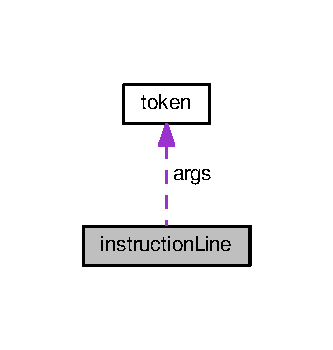
\includegraphics[width=160pt]{structinstruction_line__coll__graph}
\end{center}
\end{figure}
\subsection*{Atributos Públicos}
\begin{DoxyCompactItemize}
\item 
\hyperlink{languagedefinition_8h_a1830ff5737e4f1610e975ee2aa489206}{Instruction\-Code} \hyperlink{structinstruction_line_a309feca274873683d12f90cf0bd81780}{opcode}
\item 
\hyperlink{structtoken}{token} $\ast$ \hyperlink{structinstruction_line_ab6b4be43f89da78d09a9469f952435c7}{args}
\begin{DoxyCompactList}\small\item\em Vetor de parâmetros. \end{DoxyCompactList}\end{DoxyCompactItemize}


\subsection{Descrição detalhada}
Instrução a ser executada com parâmetros 

Definido na linha 48 do ficheiro lexer.\-h.



\subsection{Documentação dos dados membro}
\hypertarget{structinstruction_line_ab6b4be43f89da78d09a9469f952435c7}{\index{instruction\-Line@{instruction\-Line}!args@{args}}
\index{args@{args}!instructionLine@{instruction\-Line}}
\subsubsection[{args}]{\setlength{\rightskip}{0pt plus 5cm}{\bf token}$\ast$ instruction\-Line\-::args}}\label{structinstruction_line_ab6b4be43f89da78d09a9469f952435c7}


Vetor de parâmetros. 



Definido na linha 50 do ficheiro lexer.\-h.

\hypertarget{structinstruction_line_a309feca274873683d12f90cf0bd81780}{\index{instruction\-Line@{instruction\-Line}!opcode@{opcode}}
\index{opcode@{opcode}!instructionLine@{instruction\-Line}}
\subsubsection[{opcode}]{\setlength{\rightskip}{0pt plus 5cm}{\bf Instruction\-Code} instruction\-Line\-::opcode}}\label{structinstruction_line_a309feca274873683d12f90cf0bd81780}


Definido na linha 49 do ficheiro lexer.\-h.



A documentação para esta estrutura foi gerada a partir do seguinte ficheiro\-:\begin{DoxyCompactItemize}
\item 
\hyperlink{lexer_8h}{lexer.\-h}\end{DoxyCompactItemize}

\hypertarget{structtoken}{\section{Referência à estrutura token}
\label{structtoken}\index{token@{token}}
}


{\ttfamily \#include $<$lexer.\-h$>$}

\subsection*{Atributos Públicos}
\begin{DoxyCompactItemize}
\item 
\hyperlink{lexer_8h_aa520fbf142ba1e7e659590c07da31921}{Token\-Type} \hyperlink{structtoken_a0ccfb094c0dce37e1bae7d990c06cc92}{type}
\item 
std\-::string \hyperlink{structtoken_a2150b4d92215b15d0c62c40cafd407ba}{string}
\end{DoxyCompactItemize}


\subsection{Descrição detalhada}
Token identificado junto do conteúdo 

Definido na linha 36 do ficheiro lexer.\-h.



\subsection{Documentação dos dados membro}
\hypertarget{structtoken_a2150b4d92215b15d0c62c40cafd407ba}{\index{token@{token}!string@{string}}
\index{string@{string}!token@{token}}
\subsubsection[{string}]{\setlength{\rightskip}{0pt plus 5cm}std\-::string token\-::string}}\label{structtoken_a2150b4d92215b15d0c62c40cafd407ba}


Definido na linha 38 do ficheiro lexer.\-h.

\hypertarget{structtoken_a0ccfb094c0dce37e1bae7d990c06cc92}{\index{token@{token}!type@{type}}
\index{type@{type}!token@{token}}
\subsubsection[{type}]{\setlength{\rightskip}{0pt plus 5cm}{\bf Token\-Type} token\-::type}}\label{structtoken_a0ccfb094c0dce37e1bae7d990c06cc92}


Definido na linha 37 do ficheiro lexer.\-h.



A documentação para esta estrutura foi gerada a partir do seguinte ficheiro\-:\begin{DoxyCompactItemize}
\item 
\hyperlink{lexer_8h}{lexer.\-h}\end{DoxyCompactItemize}

\chapter{Documentação do ficheiro}
\hypertarget{assembler_8cpp}{\section{Referência ao ficheiro assembler.\-cpp}
\label{assembler_8cpp}\index{assembler.\-cpp@{assembler.\-cpp}}
}
{\ttfamily \#include $<$stdio.\-h$>$}\\*
{\ttfamily \#include $<$iostream$>$}\\*
{\ttfamily \#include $<$fstream$>$}\\*
{\ttfamily \#include $<$string$>$}\\*
{\ttfamily \#include $<$algorithm$>$}\\*
{\ttfamily \#include $<$vector$>$}\\*
{\ttfamily \#include $<$string.\-h$>$}\\*
{\ttfamily \#include \char`\"{}msgs\-\_\-pt.\-h\char`\"{}}\\*
{\ttfamily \#include \char`\"{}assembler.\-h\char`\"{}}\\*
{\ttfamily \#include \char`\"{}lexer.\-h\char`\"{}}\\*
{\ttfamily \#include \char`\"{}parser.\-h\char`\"{}}\\*
Diagrama de dependências de inclusão para assembler.\-cpp\-:
\nopagebreak
\begin{figure}[H]
\begin{center}
\leavevmode
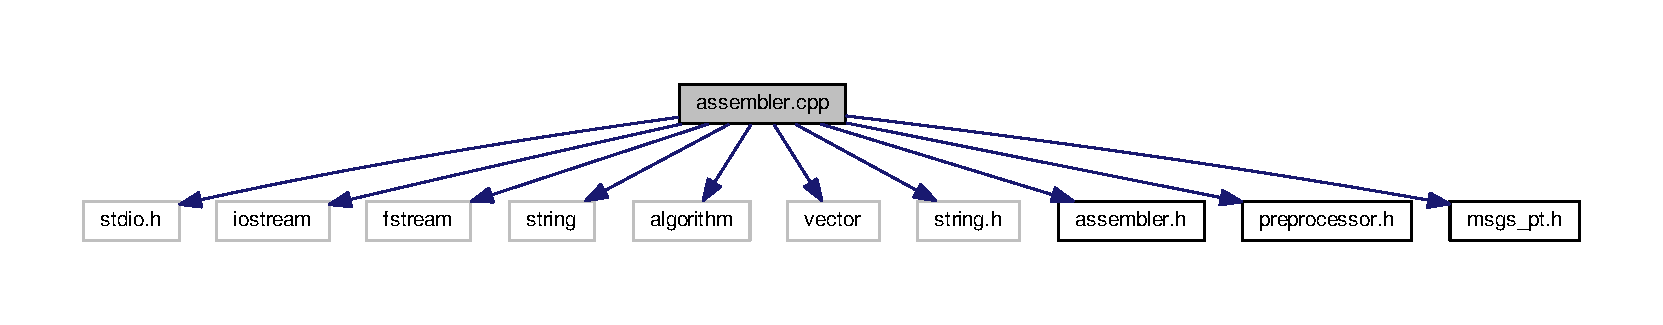
\includegraphics[width=350pt]{assembler_8cpp__incl}
\end{center}
\end{figure}
\subsection*{Funções}
\begin{DoxyCompactItemize}
\item 
int \hyperlink{assembler_8cpp_a368a4f7b83093ab74e79be4ceeb11e3d}{assembler} (int argc, char $\ast$argv\mbox{[}$\,$\mbox{]})
\end{DoxyCompactItemize}


\subsection{Documentação das funções}
\hypertarget{assembler_8cpp_a368a4f7b83093ab74e79be4ceeb11e3d}{\index{assembler.\-cpp@{assembler.\-cpp}!assembler@{assembler}}
\index{assembler@{assembler}!assembler.cpp@{assembler.\-cpp}}
\subsubsection[{assembler}]{\setlength{\rightskip}{0pt plus 5cm}int assembler (
\begin{DoxyParamCaption}
\item[{int}]{argc, }
\item[{char $\ast$}]{argv\mbox{[}$\,$\mbox{]}}
\end{DoxyParamCaption}
)}}\label{assembler_8cpp_a368a4f7b83093ab74e79be4ceeb11e3d}
Montador

\begin{DoxyAuthor}{Autor}
Rafael e João Pedro Franch 
\end{DoxyAuthor}
$<$ Tabela de Tokens

$<$ Tabela de Token 

Definido na linha 22 do ficheiro assembler.\-cpp.



Grafo de chamadas desta função\-:\nopagebreak
\begin{figure}[H]
\begin{center}
\leavevmode
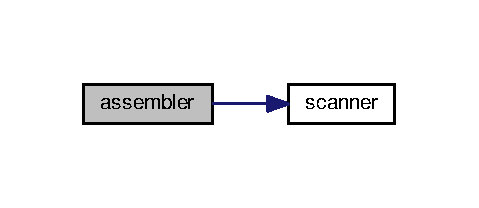
\includegraphics[width=230pt]{assembler_8cpp_a368a4f7b83093ab74e79be4ceeb11e3d_cgraph}
\end{center}
\end{figure}




Este é o diagrama das funções que utilizam esta função\-:\nopagebreak
\begin{figure}[H]
\begin{center}
\leavevmode
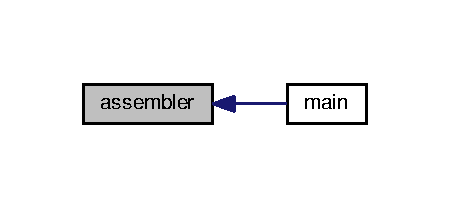
\includegraphics[width=216pt]{assembler_8cpp_a368a4f7b83093ab74e79be4ceeb11e3d_icgraph}
\end{center}
\end{figure}



\hypertarget{assembler_8h}{\section{Referência ao ficheiro assembler.\-h}
\label{assembler_8h}\index{assembler.\-h@{assembler.\-h}}
}
Este grafo mostra quais são os ficheiros que incluem directamente ou indirectamente este ficheiro\-:\nopagebreak
\begin{figure}[H]
\begin{center}
\leavevmode
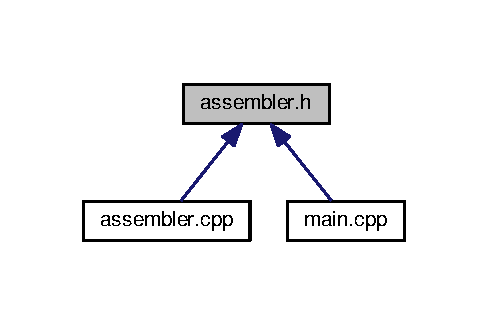
\includegraphics[width=234pt]{assembler_8h__dep__incl}
\end{center}
\end{figure}
\subsection*{Macros}
\begin{DoxyCompactItemize}
\item 
\#define \hyperlink{assembler_8h_a7aa29864c6fc48f21d74ba8b56b95018}{D\-E\-B\-U\-G\-\_\-\-A\-S\-S\-E\-M\-B\-L\-E\-R}~0
\end{DoxyCompactItemize}
\subsection*{Enumerações}
\begin{DoxyCompactItemize}
\item 
enum \hyperlink{assembler_8h_adee5669ba62dff676189189a4d6792e1}{Section\-Mode} \{ \hyperlink{assembler_8h_adee5669ba62dff676189189a4d6792e1a6d6def53fde0f7bd1cf47257d4393f55}{S\-E\-C\-T\-I\-O\-N\-\_\-\-N\-O\-N\-E} = 0, 
\hyperlink{assembler_8h_adee5669ba62dff676189189a4d6792e1ab8fff023d5919c18193cc1399d7a4218}{S\-E\-C\-T\-I\-O\-N\-\_\-\-T\-E\-X\-T} = 1, 
\hyperlink{assembler_8h_adee5669ba62dff676189189a4d6792e1adaf228104a57e890449b7c64c5c79069}{S\-E\-C\-T\-I\-O\-N\-\_\-\-D\-A\-T\-A} = 2
 \}
\end{DoxyCompactItemize}
\subsection*{Funções}
\begin{DoxyCompactItemize}
\item 
int \hyperlink{assembler_8h_a368a4f7b83093ab74e79be4ceeb11e3d}{assembler} (int argc, char $\ast$argv\mbox{[}$\,$\mbox{]})
\end{DoxyCompactItemize}


\subsection{Documentação das macros}
\hypertarget{assembler_8h_a7aa29864c6fc48f21d74ba8b56b95018}{\index{assembler.\-h@{assembler.\-h}!D\-E\-B\-U\-G\-\_\-\-A\-S\-S\-E\-M\-B\-L\-E\-R@{D\-E\-B\-U\-G\-\_\-\-A\-S\-S\-E\-M\-B\-L\-E\-R}}
\index{D\-E\-B\-U\-G\-\_\-\-A\-S\-S\-E\-M\-B\-L\-E\-R@{D\-E\-B\-U\-G\-\_\-\-A\-S\-S\-E\-M\-B\-L\-E\-R}!assembler.h@{assembler.\-h}}
\subsubsection[{D\-E\-B\-U\-G\-\_\-\-A\-S\-S\-E\-M\-B\-L\-E\-R}]{\setlength{\rightskip}{0pt plus 5cm}\#define D\-E\-B\-U\-G\-\_\-\-A\-S\-S\-E\-M\-B\-L\-E\-R~0}}\label{assembler_8h_a7aa29864c6fc48f21d74ba8b56b95018}


Definido na linha 4 do ficheiro assembler.\-h.



\subsection{Documentação dos valores da enumeração}
\hypertarget{assembler_8h_adee5669ba62dff676189189a4d6792e1}{\index{assembler.\-h@{assembler.\-h}!Section\-Mode@{Section\-Mode}}
\index{Section\-Mode@{Section\-Mode}!assembler.h@{assembler.\-h}}
\subsubsection[{Section\-Mode}]{\setlength{\rightskip}{0pt plus 5cm}enum {\bf Section\-Mode}}}\label{assembler_8h_adee5669ba62dff676189189a4d6792e1}
\begin{Desc}
\item[Valores da enumeração]\par
\begin{description}
\index{S\-E\-C\-T\-I\-O\-N\-\_\-\-N\-O\-N\-E@{S\-E\-C\-T\-I\-O\-N\-\_\-\-N\-O\-N\-E}!assembler.\-h@{assembler.\-h}}\index{assembler.\-h@{assembler.\-h}!S\-E\-C\-T\-I\-O\-N\-\_\-\-N\-O\-N\-E@{S\-E\-C\-T\-I\-O\-N\-\_\-\-N\-O\-N\-E}}\item[{\em 
\hypertarget{assembler_8h_adee5669ba62dff676189189a4d6792e1a6d6def53fde0f7bd1cf47257d4393f55}{S\-E\-C\-T\-I\-O\-N\-\_\-\-N\-O\-N\-E}\label{assembler_8h_adee5669ba62dff676189189a4d6792e1a6d6def53fde0f7bd1cf47257d4393f55}
}]\index{S\-E\-C\-T\-I\-O\-N\-\_\-\-T\-E\-X\-T@{S\-E\-C\-T\-I\-O\-N\-\_\-\-T\-E\-X\-T}!assembler.\-h@{assembler.\-h}}\index{assembler.\-h@{assembler.\-h}!S\-E\-C\-T\-I\-O\-N\-\_\-\-T\-E\-X\-T@{S\-E\-C\-T\-I\-O\-N\-\_\-\-T\-E\-X\-T}}\item[{\em 
\hypertarget{assembler_8h_adee5669ba62dff676189189a4d6792e1ab8fff023d5919c18193cc1399d7a4218}{S\-E\-C\-T\-I\-O\-N\-\_\-\-T\-E\-X\-T}\label{assembler_8h_adee5669ba62dff676189189a4d6792e1ab8fff023d5919c18193cc1399d7a4218}
}]\index{S\-E\-C\-T\-I\-O\-N\-\_\-\-D\-A\-T\-A@{S\-E\-C\-T\-I\-O\-N\-\_\-\-D\-A\-T\-A}!assembler.\-h@{assembler.\-h}}\index{assembler.\-h@{assembler.\-h}!S\-E\-C\-T\-I\-O\-N\-\_\-\-D\-A\-T\-A@{S\-E\-C\-T\-I\-O\-N\-\_\-\-D\-A\-T\-A}}\item[{\em 
\hypertarget{assembler_8h_adee5669ba62dff676189189a4d6792e1adaf228104a57e890449b7c64c5c79069}{S\-E\-C\-T\-I\-O\-N\-\_\-\-D\-A\-T\-A}\label{assembler_8h_adee5669ba62dff676189189a4d6792e1adaf228104a57e890449b7c64c5c79069}
}]\end{description}
\end{Desc}


Definido na linha 7 do ficheiro assembler.\-h.



\subsection{Documentação das funções}
\hypertarget{assembler_8h_a368a4f7b83093ab74e79be4ceeb11e3d}{\index{assembler.\-h@{assembler.\-h}!assembler@{assembler}}
\index{assembler@{assembler}!assembler.h@{assembler.\-h}}
\subsubsection[{assembler}]{\setlength{\rightskip}{0pt plus 5cm}int assembler (
\begin{DoxyParamCaption}
\item[{int}]{argc, }
\item[{char $\ast$}]{argv\mbox{[}$\,$\mbox{]}}
\end{DoxyParamCaption}
)}}\label{assembler_8h_a368a4f7b83093ab74e79be4ceeb11e3d}
Montador

\begin{DoxyAuthor}{Autor}
Rafael e João Pedro Franch 
\end{DoxyAuthor}
$<$ Tabela de Tokens

\begin{DoxyRefDesc}{Tarefa}
\item[\hyperlink{todo__todo000001}{Tarefa}]Modificar para permitir completar tabela ao final da passagem \end{DoxyRefDesc}


\begin{DoxyRefDesc}{Tarefa}
\item[\hyperlink{todo__todo000002}{Tarefa}]Modificar para permitir completar tabela ao final da passagem \end{DoxyRefDesc}


\begin{DoxyRefDesc}{Tarefa}
\item[\hyperlink{todo__todo000003}{Tarefa}]Modificar para permitir completar tabela ao final da passagem \end{DoxyRefDesc}


\begin{DoxyRefDesc}{Tarefa}
\item[\hyperlink{todo__todo000004}{Tarefa}]Modificar para permitir completar tabela ao final da passagem \end{DoxyRefDesc}


\begin{DoxyRefDesc}{Bug}
\item[\hyperlink{bug__bug000001}{Bug}]começando contagem a partir do 1 ao invés do 0 \end{DoxyRefDesc}


\begin{DoxyRefDesc}{Tarefa}
\item[\hyperlink{todo__todo000005}{Tarefa}]Modificar para permitir completar tabela ao final da passagem \end{DoxyRefDesc}


\begin{DoxyRefDesc}{Tarefa}
\item[\hyperlink{todo__todo000006}{Tarefa}]Modificar para permitir completar tabela ao final da passagem \end{DoxyRefDesc}


\begin{DoxyRefDesc}{Tarefa}
\item[\hyperlink{todo__todo000007}{Tarefa}]Modificar para permitir completar tabela ao final da passagem \end{DoxyRefDesc}


\begin{DoxyRefDesc}{Tarefa}
\item[\hyperlink{todo__todo000008}{Tarefa}]Modificar Programa para permitir identificar linha do erro \end{DoxyRefDesc}


\begin{DoxyRefDesc}{Tarefa}
\item[\hyperlink{todo__todo000009}{Tarefa}]Modificar Programa para permitir identificar linha do erro \end{DoxyRefDesc}


Definido na linha 23 do ficheiro assembler.\-cpp.



Grafo de chamadas desta função\-:
\nopagebreak
\begin{figure}[H]
\begin{center}
\leavevmode
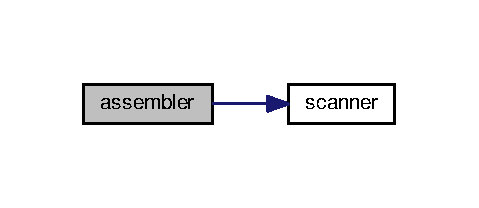
\includegraphics[width=288pt]{assembler_8h_a368a4f7b83093ab74e79be4ceeb11e3d_cgraph}
\end{center}
\end{figure}




Este é o diagrama das funções que utilizam esta função\-:\nopagebreak
\begin{figure}[H]
\begin{center}
\leavevmode
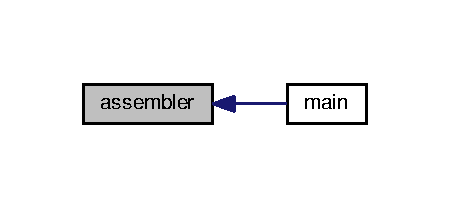
\includegraphics[width=216pt]{assembler_8h_a368a4f7b83093ab74e79be4ceeb11e3d_icgraph}
\end{center}
\end{figure}



\hypertarget{languagedefinition_8h}{\section{Referência ao ficheiro languagedefinition.\-h}
\label{languagedefinition_8h}\index{languagedefinition.\-h@{languagedefinition.\-h}}
}
Este grafo mostra quais são os ficheiros que incluem directamente ou indirectamente este ficheiro\-:
\nopagebreak
\begin{figure}[H]
\begin{center}
\leavevmode
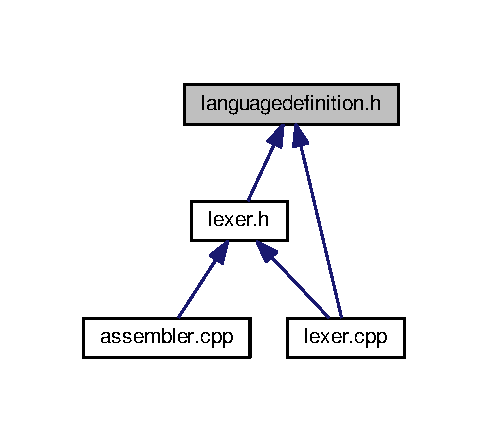
\includegraphics[width=344pt]{languagedefinition_8h__dep__incl}
\end{center}
\end{figure}
\subsection*{Macros}
\begin{DoxyCompactItemize}
\item 
\#define \hyperlink{languagedefinition_8h_ac56a94e3a6c9fcfb2f0fe4e6f88bb841}{I\-N\-S\-T\-R\-U\-C\-T\-I\-O\-N\-S\-\_\-\-N\-U\-M\-B\-E\-R}~24
\end{DoxyCompactItemize}
\subsection*{Enumerações}
\begin{DoxyCompactItemize}
\item 
enum \hyperlink{languagedefinition_8h_a1830ff5737e4f1610e975ee2aa489206}{Instruction\-Code} \{ \\*
\hyperlink{languagedefinition_8h_a1830ff5737e4f1610e975ee2aa489206acfcf145f2788bf340ff3f3098bc54909}{A\-D\-D} = 1, 
\hyperlink{languagedefinition_8h_a1830ff5737e4f1610e975ee2aa489206a12b733d4941495e86811fe6ceeeff9da}{S\-U\-B} = 2, 
\hyperlink{languagedefinition_8h_a1830ff5737e4f1610e975ee2aa489206a18a2956fb463e60c1a099d6d69e2c0ef}{M\-U\-L\-T} = 3, 
\hyperlink{languagedefinition_8h_a1830ff5737e4f1610e975ee2aa489206a8565f0d60c3ba6d468661c49d86e9744}{D\-I\-V} = 4, 
\\*
\hyperlink{languagedefinition_8h_a1830ff5737e4f1610e975ee2aa489206a227d95ecea3ff1219ddb58bb03d17d5a}{J\-M\-P} = 5, 
\hyperlink{languagedefinition_8h_a1830ff5737e4f1610e975ee2aa489206a5ad8848077462c4715134595407577b3}{J\-M\-P\-N} = 6, 
\hyperlink{languagedefinition_8h_a1830ff5737e4f1610e975ee2aa489206aabcd878e992d92075d914162254aa565}{J\-M\-P\-P} = 7, 
\hyperlink{languagedefinition_8h_a1830ff5737e4f1610e975ee2aa489206a73b248f18b6c36a4221e87628722d84a}{J\-M\-P\-Z} = 8, 
\\*
\hyperlink{languagedefinition_8h_a1830ff5737e4f1610e975ee2aa489206aba6788019f0f871f0aefcd5644635785}{C\-O\-P\-Y} = 9, 
\hyperlink{languagedefinition_8h_a1830ff5737e4f1610e975ee2aa489206a972dbcdf74cff71e20bdcfb53be9c391}{L\-O\-A\-D} = 10, 
\hyperlink{languagedefinition_8h_a1830ff5737e4f1610e975ee2aa489206afeb01cb4572ba190cd7932e49446c480}{S\-T\-O\-R\-E} = 11, 
\hyperlink{languagedefinition_8h_a1830ff5737e4f1610e975ee2aa489206ae310c909d76b003d016bef8bdf16936a}{I\-N\-P\-U\-T} = 12, 
\\*
\hyperlink{languagedefinition_8h_a1830ff5737e4f1610e975ee2aa489206a2ab08d3e103968f5f4f26b66a52e99d6}{O\-U\-T\-P\-U\-T} = 13, 
\hyperlink{languagedefinition_8h_a1830ff5737e4f1610e975ee2aa489206a679ee5320d66c8322e310daeb2ee99b8}{S\-T\-O\-P} = 14, 
\hyperlink{languagedefinition_8h_a1830ff5737e4f1610e975ee2aa489206acb7227be6a36b93e485b62e3acddae51}{S\-E\-C\-T\-I\-O\-N} = 15, 
\hyperlink{languagedefinition_8h_a1830ff5737e4f1610e975ee2aa489206aacb2c772b330b152747db851e79ecfb9}{S\-P\-A\-C\-E0} = 16, 
\\*
\hyperlink{languagedefinition_8h_a1830ff5737e4f1610e975ee2aa489206a0b7afa414f09ecc4d88ad562a013db6d}{S\-P\-A\-C\-E1} = 17, 
\hyperlink{languagedefinition_8h_a1830ff5737e4f1610e975ee2aa489206a3d044162d972156d897cea80f216b9ca}{C\-O\-N\-S\-T} = 18, 
\hyperlink{languagedefinition_8h_a1830ff5737e4f1610e975ee2aa489206aa7db066a95277c0ad6aedf5eb9879072}{E\-Q\-U} = 19, 
\hyperlink{languagedefinition_8h_a1830ff5737e4f1610e975ee2aa489206a252802eda493fb6b4a279c4452acb547}{I\-F} = 20, 
\\*
\hyperlink{languagedefinition_8h_a1830ff5737e4f1610e975ee2aa489206a3d1738a931468da77c233f1126436b81}{M\-A\-C\-R\-O} = 21, 
\hyperlink{languagedefinition_8h_a1830ff5737e4f1610e975ee2aa489206ad0fc1697471abaa771ad0c5db5be85f0}{E\-N\-D\-M\-A\-C\-R\-O} = 22, 
\hyperlink{languagedefinition_8h_a1830ff5737e4f1610e975ee2aa489206a368db50032da622d4c456ef7eaf9cb67}{B\-E\-G\-I\-N} = 23, 
\hyperlink{languagedefinition_8h_a1830ff5737e4f1610e975ee2aa489206adc6f24fd6915a3f2786a1b7045406924}{E\-N\-D} = 24
 \}
\end{DoxyCompactItemize}
\subsection*{Variáveis}
\begin{DoxyCompactItemize}
\item 
static const char $\ast$ \hyperlink{languagedefinition_8h_a40869f6bf4eb1263aeccc9feb241d620}{Instrution\-String} \mbox{[}$\,$\mbox{]}
\item 
static const int \hyperlink{languagedefinition_8h_a9b3f3be9136926d1cf555ff0820a78d0}{Instruction\-Arg\-Number} \mbox{[}$\,$\mbox{]}
\end{DoxyCompactItemize}


\subsection{Descrição detalhada}
\#brief Definições da liguagem assembly

\begin{DoxyAuthor}{Autores}
Rafael Lima 
\end{DoxyAuthor}


Definido no ficheiro \hyperlink{languagedefinition_8h_source}{languagedefinition.\-h}.



\subsection{Documentação das macros}
\hypertarget{languagedefinition_8h_ac56a94e3a6c9fcfb2f0fe4e6f88bb841}{\index{languagedefinition.\-h@{languagedefinition.\-h}!I\-N\-S\-T\-R\-U\-C\-T\-I\-O\-N\-S\-\_\-\-N\-U\-M\-B\-E\-R@{I\-N\-S\-T\-R\-U\-C\-T\-I\-O\-N\-S\-\_\-\-N\-U\-M\-B\-E\-R}}
\index{I\-N\-S\-T\-R\-U\-C\-T\-I\-O\-N\-S\-\_\-\-N\-U\-M\-B\-E\-R@{I\-N\-S\-T\-R\-U\-C\-T\-I\-O\-N\-S\-\_\-\-N\-U\-M\-B\-E\-R}!languagedefinition.h@{languagedefinition.\-h}}
\subsubsection[{I\-N\-S\-T\-R\-U\-C\-T\-I\-O\-N\-S\-\_\-\-N\-U\-M\-B\-E\-R}]{\setlength{\rightskip}{0pt plus 5cm}\#define I\-N\-S\-T\-R\-U\-C\-T\-I\-O\-N\-S\-\_\-\-N\-U\-M\-B\-E\-R~24}}\label{languagedefinition_8h_ac56a94e3a6c9fcfb2f0fe4e6f88bb841}


Definido na linha 43 do ficheiro languagedefinition.\-h.



\subsection{Documentação dos valores da enumeração}
\hypertarget{languagedefinition_8h_a1830ff5737e4f1610e975ee2aa489206}{\index{languagedefinition.\-h@{languagedefinition.\-h}!Instruction\-Code@{Instruction\-Code}}
\index{Instruction\-Code@{Instruction\-Code}!languagedefinition.h@{languagedefinition.\-h}}
\subsubsection[{Instruction\-Code}]{\setlength{\rightskip}{0pt plus 5cm}enum {\bf Instruction\-Code}}}\label{languagedefinition_8h_a1830ff5737e4f1610e975ee2aa489206}
Código das instruções \begin{DoxyRefDesc}{Tarefa}
\item[\hyperlink{todo__todo000008}{Tarefa}]Alterar Opcodes para compatibilidade com simulador 

Separar Instruções de Diretivas em tipos distintos \end{DoxyRefDesc}
\begin{Desc}
\item[Valores da enumeração]\par
\begin{description}
\index{A\-D\-D@{A\-D\-D}!languagedefinition.\-h@{languagedefinition.\-h}}\index{languagedefinition.\-h@{languagedefinition.\-h}!A\-D\-D@{A\-D\-D}}\item[{\em 
\hypertarget{languagedefinition_8h_a1830ff5737e4f1610e975ee2aa489206acfcf145f2788bf340ff3f3098bc54909}{A\-D\-D}\label{languagedefinition_8h_a1830ff5737e4f1610e975ee2aa489206acfcf145f2788bf340ff3f3098bc54909}
}]\index{S\-U\-B@{S\-U\-B}!languagedefinition.\-h@{languagedefinition.\-h}}\index{languagedefinition.\-h@{languagedefinition.\-h}!S\-U\-B@{S\-U\-B}}\item[{\em 
\hypertarget{languagedefinition_8h_a1830ff5737e4f1610e975ee2aa489206a12b733d4941495e86811fe6ceeeff9da}{S\-U\-B}\label{languagedefinition_8h_a1830ff5737e4f1610e975ee2aa489206a12b733d4941495e86811fe6ceeeff9da}
}]\index{M\-U\-L\-T@{M\-U\-L\-T}!languagedefinition.\-h@{languagedefinition.\-h}}\index{languagedefinition.\-h@{languagedefinition.\-h}!M\-U\-L\-T@{M\-U\-L\-T}}\item[{\em 
\hypertarget{languagedefinition_8h_a1830ff5737e4f1610e975ee2aa489206a18a2956fb463e60c1a099d6d69e2c0ef}{M\-U\-L\-T}\label{languagedefinition_8h_a1830ff5737e4f1610e975ee2aa489206a18a2956fb463e60c1a099d6d69e2c0ef}
}]\index{D\-I\-V@{D\-I\-V}!languagedefinition.\-h@{languagedefinition.\-h}}\index{languagedefinition.\-h@{languagedefinition.\-h}!D\-I\-V@{D\-I\-V}}\item[{\em 
\hypertarget{languagedefinition_8h_a1830ff5737e4f1610e975ee2aa489206a8565f0d60c3ba6d468661c49d86e9744}{D\-I\-V}\label{languagedefinition_8h_a1830ff5737e4f1610e975ee2aa489206a8565f0d60c3ba6d468661c49d86e9744}
}]\index{J\-M\-P@{J\-M\-P}!languagedefinition.\-h@{languagedefinition.\-h}}\index{languagedefinition.\-h@{languagedefinition.\-h}!J\-M\-P@{J\-M\-P}}\item[{\em 
\hypertarget{languagedefinition_8h_a1830ff5737e4f1610e975ee2aa489206a227d95ecea3ff1219ddb58bb03d17d5a}{J\-M\-P}\label{languagedefinition_8h_a1830ff5737e4f1610e975ee2aa489206a227d95ecea3ff1219ddb58bb03d17d5a}
}]\index{J\-M\-P\-N@{J\-M\-P\-N}!languagedefinition.\-h@{languagedefinition.\-h}}\index{languagedefinition.\-h@{languagedefinition.\-h}!J\-M\-P\-N@{J\-M\-P\-N}}\item[{\em 
\hypertarget{languagedefinition_8h_a1830ff5737e4f1610e975ee2aa489206a5ad8848077462c4715134595407577b3}{J\-M\-P\-N}\label{languagedefinition_8h_a1830ff5737e4f1610e975ee2aa489206a5ad8848077462c4715134595407577b3}
}]\index{J\-M\-P\-P@{J\-M\-P\-P}!languagedefinition.\-h@{languagedefinition.\-h}}\index{languagedefinition.\-h@{languagedefinition.\-h}!J\-M\-P\-P@{J\-M\-P\-P}}\item[{\em 
\hypertarget{languagedefinition_8h_a1830ff5737e4f1610e975ee2aa489206aabcd878e992d92075d914162254aa565}{J\-M\-P\-P}\label{languagedefinition_8h_a1830ff5737e4f1610e975ee2aa489206aabcd878e992d92075d914162254aa565}
}]\index{J\-M\-P\-Z@{J\-M\-P\-Z}!languagedefinition.\-h@{languagedefinition.\-h}}\index{languagedefinition.\-h@{languagedefinition.\-h}!J\-M\-P\-Z@{J\-M\-P\-Z}}\item[{\em 
\hypertarget{languagedefinition_8h_a1830ff5737e4f1610e975ee2aa489206a73b248f18b6c36a4221e87628722d84a}{J\-M\-P\-Z}\label{languagedefinition_8h_a1830ff5737e4f1610e975ee2aa489206a73b248f18b6c36a4221e87628722d84a}
}]\index{C\-O\-P\-Y@{C\-O\-P\-Y}!languagedefinition.\-h@{languagedefinition.\-h}}\index{languagedefinition.\-h@{languagedefinition.\-h}!C\-O\-P\-Y@{C\-O\-P\-Y}}\item[{\em 
\hypertarget{languagedefinition_8h_a1830ff5737e4f1610e975ee2aa489206aba6788019f0f871f0aefcd5644635785}{C\-O\-P\-Y}\label{languagedefinition_8h_a1830ff5737e4f1610e975ee2aa489206aba6788019f0f871f0aefcd5644635785}
}]\index{L\-O\-A\-D@{L\-O\-A\-D}!languagedefinition.\-h@{languagedefinition.\-h}}\index{languagedefinition.\-h@{languagedefinition.\-h}!L\-O\-A\-D@{L\-O\-A\-D}}\item[{\em 
\hypertarget{languagedefinition_8h_a1830ff5737e4f1610e975ee2aa489206a972dbcdf74cff71e20bdcfb53be9c391}{L\-O\-A\-D}\label{languagedefinition_8h_a1830ff5737e4f1610e975ee2aa489206a972dbcdf74cff71e20bdcfb53be9c391}
}]\index{S\-T\-O\-R\-E@{S\-T\-O\-R\-E}!languagedefinition.\-h@{languagedefinition.\-h}}\index{languagedefinition.\-h@{languagedefinition.\-h}!S\-T\-O\-R\-E@{S\-T\-O\-R\-E}}\item[{\em 
\hypertarget{languagedefinition_8h_a1830ff5737e4f1610e975ee2aa489206afeb01cb4572ba190cd7932e49446c480}{S\-T\-O\-R\-E}\label{languagedefinition_8h_a1830ff5737e4f1610e975ee2aa489206afeb01cb4572ba190cd7932e49446c480}
}]\index{I\-N\-P\-U\-T@{I\-N\-P\-U\-T}!languagedefinition.\-h@{languagedefinition.\-h}}\index{languagedefinition.\-h@{languagedefinition.\-h}!I\-N\-P\-U\-T@{I\-N\-P\-U\-T}}\item[{\em 
\hypertarget{languagedefinition_8h_a1830ff5737e4f1610e975ee2aa489206ae310c909d76b003d016bef8bdf16936a}{I\-N\-P\-U\-T}\label{languagedefinition_8h_a1830ff5737e4f1610e975ee2aa489206ae310c909d76b003d016bef8bdf16936a}
}]\index{O\-U\-T\-P\-U\-T@{O\-U\-T\-P\-U\-T}!languagedefinition.\-h@{languagedefinition.\-h}}\index{languagedefinition.\-h@{languagedefinition.\-h}!O\-U\-T\-P\-U\-T@{O\-U\-T\-P\-U\-T}}\item[{\em 
\hypertarget{languagedefinition_8h_a1830ff5737e4f1610e975ee2aa489206a2ab08d3e103968f5f4f26b66a52e99d6}{O\-U\-T\-P\-U\-T}\label{languagedefinition_8h_a1830ff5737e4f1610e975ee2aa489206a2ab08d3e103968f5f4f26b66a52e99d6}
}]\index{S\-T\-O\-P@{S\-T\-O\-P}!languagedefinition.\-h@{languagedefinition.\-h}}\index{languagedefinition.\-h@{languagedefinition.\-h}!S\-T\-O\-P@{S\-T\-O\-P}}\item[{\em 
\hypertarget{languagedefinition_8h_a1830ff5737e4f1610e975ee2aa489206a679ee5320d66c8322e310daeb2ee99b8}{S\-T\-O\-P}\label{languagedefinition_8h_a1830ff5737e4f1610e975ee2aa489206a679ee5320d66c8322e310daeb2ee99b8}
}]\index{S\-E\-C\-T\-I\-O\-N@{S\-E\-C\-T\-I\-O\-N}!languagedefinition.\-h@{languagedefinition.\-h}}\index{languagedefinition.\-h@{languagedefinition.\-h}!S\-E\-C\-T\-I\-O\-N@{S\-E\-C\-T\-I\-O\-N}}\item[{\em 
\hypertarget{languagedefinition_8h_a1830ff5737e4f1610e975ee2aa489206acb7227be6a36b93e485b62e3acddae51}{S\-E\-C\-T\-I\-O\-N}\label{languagedefinition_8h_a1830ff5737e4f1610e975ee2aa489206acb7227be6a36b93e485b62e3acddae51}
}]\index{S\-P\-A\-C\-E0@{S\-P\-A\-C\-E0}!languagedefinition.\-h@{languagedefinition.\-h}}\index{languagedefinition.\-h@{languagedefinition.\-h}!S\-P\-A\-C\-E0@{S\-P\-A\-C\-E0}}\item[{\em 
\hypertarget{languagedefinition_8h_a1830ff5737e4f1610e975ee2aa489206aacb2c772b330b152747db851e79ecfb9}{S\-P\-A\-C\-E0}\label{languagedefinition_8h_a1830ff5737e4f1610e975ee2aa489206aacb2c772b330b152747db851e79ecfb9}
}]\index{S\-P\-A\-C\-E1@{S\-P\-A\-C\-E1}!languagedefinition.\-h@{languagedefinition.\-h}}\index{languagedefinition.\-h@{languagedefinition.\-h}!S\-P\-A\-C\-E1@{S\-P\-A\-C\-E1}}\item[{\em 
\hypertarget{languagedefinition_8h_a1830ff5737e4f1610e975ee2aa489206a0b7afa414f09ecc4d88ad562a013db6d}{S\-P\-A\-C\-E1}\label{languagedefinition_8h_a1830ff5737e4f1610e975ee2aa489206a0b7afa414f09ecc4d88ad562a013db6d}
}]\index{C\-O\-N\-S\-T@{C\-O\-N\-S\-T}!languagedefinition.\-h@{languagedefinition.\-h}}\index{languagedefinition.\-h@{languagedefinition.\-h}!C\-O\-N\-S\-T@{C\-O\-N\-S\-T}}\item[{\em 
\hypertarget{languagedefinition_8h_a1830ff5737e4f1610e975ee2aa489206a3d044162d972156d897cea80f216b9ca}{C\-O\-N\-S\-T}\label{languagedefinition_8h_a1830ff5737e4f1610e975ee2aa489206a3d044162d972156d897cea80f216b9ca}
}]\index{E\-Q\-U@{E\-Q\-U}!languagedefinition.\-h@{languagedefinition.\-h}}\index{languagedefinition.\-h@{languagedefinition.\-h}!E\-Q\-U@{E\-Q\-U}}\item[{\em 
\hypertarget{languagedefinition_8h_a1830ff5737e4f1610e975ee2aa489206aa7db066a95277c0ad6aedf5eb9879072}{E\-Q\-U}\label{languagedefinition_8h_a1830ff5737e4f1610e975ee2aa489206aa7db066a95277c0ad6aedf5eb9879072}
}]\index{I\-F@{I\-F}!languagedefinition.\-h@{languagedefinition.\-h}}\index{languagedefinition.\-h@{languagedefinition.\-h}!I\-F@{I\-F}}\item[{\em 
\hypertarget{languagedefinition_8h_a1830ff5737e4f1610e975ee2aa489206a252802eda493fb6b4a279c4452acb547}{I\-F}\label{languagedefinition_8h_a1830ff5737e4f1610e975ee2aa489206a252802eda493fb6b4a279c4452acb547}
}]\index{M\-A\-C\-R\-O@{M\-A\-C\-R\-O}!languagedefinition.\-h@{languagedefinition.\-h}}\index{languagedefinition.\-h@{languagedefinition.\-h}!M\-A\-C\-R\-O@{M\-A\-C\-R\-O}}\item[{\em 
\hypertarget{languagedefinition_8h_a1830ff5737e4f1610e975ee2aa489206a3d1738a931468da77c233f1126436b81}{M\-A\-C\-R\-O}\label{languagedefinition_8h_a1830ff5737e4f1610e975ee2aa489206a3d1738a931468da77c233f1126436b81}
}]\index{E\-N\-D\-M\-A\-C\-R\-O@{E\-N\-D\-M\-A\-C\-R\-O}!languagedefinition.\-h@{languagedefinition.\-h}}\index{languagedefinition.\-h@{languagedefinition.\-h}!E\-N\-D\-M\-A\-C\-R\-O@{E\-N\-D\-M\-A\-C\-R\-O}}\item[{\em 
\hypertarget{languagedefinition_8h_a1830ff5737e4f1610e975ee2aa489206ad0fc1697471abaa771ad0c5db5be85f0}{E\-N\-D\-M\-A\-C\-R\-O}\label{languagedefinition_8h_a1830ff5737e4f1610e975ee2aa489206ad0fc1697471abaa771ad0c5db5be85f0}
}]\index{B\-E\-G\-I\-N@{B\-E\-G\-I\-N}!languagedefinition.\-h@{languagedefinition.\-h}}\index{languagedefinition.\-h@{languagedefinition.\-h}!B\-E\-G\-I\-N@{B\-E\-G\-I\-N}}\item[{\em 
\hypertarget{languagedefinition_8h_a1830ff5737e4f1610e975ee2aa489206a368db50032da622d4c456ef7eaf9cb67}{B\-E\-G\-I\-N}\label{languagedefinition_8h_a1830ff5737e4f1610e975ee2aa489206a368db50032da622d4c456ef7eaf9cb67}
}]\index{E\-N\-D@{E\-N\-D}!languagedefinition.\-h@{languagedefinition.\-h}}\index{languagedefinition.\-h@{languagedefinition.\-h}!E\-N\-D@{E\-N\-D}}\item[{\em 
\hypertarget{languagedefinition_8h_a1830ff5737e4f1610e975ee2aa489206adc6f24fd6915a3f2786a1b7045406924}{E\-N\-D}\label{languagedefinition_8h_a1830ff5737e4f1610e975ee2aa489206adc6f24fd6915a3f2786a1b7045406924}
}]\end{description}
\end{Desc}


Definido na linha 16 do ficheiro languagedefinition.\-h.



\subsection{Documentação das variáveis}
\hypertarget{languagedefinition_8h_a9b3f3be9136926d1cf555ff0820a78d0}{\index{languagedefinition.\-h@{languagedefinition.\-h}!Instruction\-Arg\-Number@{Instruction\-Arg\-Number}}
\index{Instruction\-Arg\-Number@{Instruction\-Arg\-Number}!languagedefinition.h@{languagedefinition.\-h}}
\subsubsection[{Instruction\-Arg\-Number}]{\setlength{\rightskip}{0pt plus 5cm}const int Instruction\-Arg\-Number\mbox{[}$\,$\mbox{]}\hspace{0.3cm}{\ttfamily [static]}}}\label{languagedefinition_8h_a9b3f3be9136926d1cf555ff0820a78d0}
{\bfseries Valor inicial\-:}
\begin{DoxyCode}
= \{
    1, 
    1, 
    1, 
    1, 
    1, 
    1, 
    1, 
    1, 
    2, 
    1, 
    1, 
    1, 
    1, 
    0, 
    1, 
    0, 
    1, 
    1, 
    1, 
    1, 
    0, 
    0, 
    0, 
    0  
\}
\end{DoxyCode}
Quantidade de argumentos de cada instrução esta na mesma ordem do Instruction\mbox{[}\mbox{]} 

Definido na linha 76 do ficheiro languagedefinition.\-h.

\hypertarget{languagedefinition_8h_a40869f6bf4eb1263aeccc9feb241d620}{\index{languagedefinition.\-h@{languagedefinition.\-h}!Instrution\-String@{Instrution\-String}}
\index{Instrution\-String@{Instrution\-String}!languagedefinition.h@{languagedefinition.\-h}}
\subsubsection[{Instrution\-String}]{\setlength{\rightskip}{0pt plus 5cm}const char$\ast$ Instrution\-String\mbox{[}$\,$\mbox{]}\hspace{0.3cm}{\ttfamily [static]}}}\label{languagedefinition_8h_a40869f6bf4eb1263aeccc9feb241d620}
{\bfseries Valor inicial\-:}
\begin{DoxyCode}
= \{
  \textcolor{stringliteral}{"ADD"},
  \textcolor{stringliteral}{"SUB"},
  \textcolor{stringliteral}{"MULT"},
  \textcolor{stringliteral}{"DIV"},
  \textcolor{stringliteral}{"JMP"},
  \textcolor{stringliteral}{"JMPN"},
  \textcolor{stringliteral}{"JMPP"},
  \textcolor{stringliteral}{"JMPZ"},
  \textcolor{stringliteral}{"COPY"},
  \textcolor{stringliteral}{"LOAD"},
  \textcolor{stringliteral}{"STORE"},
  \textcolor{stringliteral}{"INPUT"},
  \textcolor{stringliteral}{"OUTPUT"},
  \textcolor{stringliteral}{"STOP"},
  \textcolor{stringliteral}{"SECTION"},
  \textcolor{stringliteral}{"SPACE"},
  \textcolor{stringliteral}{"SPACE"},
  \textcolor{stringliteral}{"CONST"},
  \textcolor{stringliteral}{"EQU"},
  \textcolor{stringliteral}{"IF"},
  \textcolor{stringliteral}{"MACRO"},
  \textcolor{stringliteral}{"ENDMACRO"},
  \textcolor{stringliteral}{"BEGIN"},
  \textcolor{stringliteral}{"END"}
\}
\end{DoxyCode}


Definido na linha 45 do ficheiro languagedefinition.\-h.


\hypertarget{lexer_8cpp}{\section{Referência ao ficheiro lexer.\-cpp}
\label{lexer_8cpp}\index{lexer.\-cpp@{lexer.\-cpp}}
}
{\ttfamily \#include $<$vector$>$}\\*
{\ttfamily \#include \char`\"{}languagedefinition.\-h\char`\"{}}\\*
{\ttfamily \#include \char`\"{}lexer.\-h\char`\"{}}\\*
Diagrama de dependências de inclusão para lexer.\-cpp\-:
\nopagebreak
\begin{figure}[H]
\begin{center}
\leavevmode
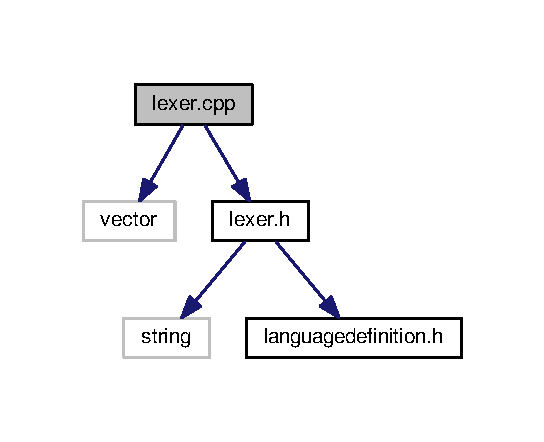
\includegraphics[width=261pt]{lexer_8cpp__incl}
\end{center}
\end{figure}
\subsection*{Funções}
\begin{DoxyCompactItemize}
\item 
\hyperlink{structtoken}{token} \hyperlink{lexer_8cpp_a63ef6d488951c4541159fe0961565c4d}{scanner} (std\-::string line, int $\ast$position)
\item 
int \hyperlink{lexer_8cpp_ac34489ced263c84198b4c0e83643ebe7}{is\-Valid\-Instruction} (string command)
\end{DoxyCompactItemize}


\subsection{Documentação das funções}
\hypertarget{lexer_8cpp_ac34489ced263c84198b4c0e83643ebe7}{\index{lexer.\-cpp@{lexer.\-cpp}!is\-Valid\-Instruction@{is\-Valid\-Instruction}}
\index{is\-Valid\-Instruction@{is\-Valid\-Instruction}!lexer.cpp@{lexer.\-cpp}}
\subsubsection[{is\-Valid\-Instruction}]{\setlength{\rightskip}{0pt plus 5cm}int is\-Valid\-Instruction (
\begin{DoxyParamCaption}
\item[{string}]{command}
\end{DoxyParamCaption}
)}}\label{lexer_8cpp_ac34489ced263c84198b4c0e83643ebe7}


Definido na linha 108 do ficheiro lexer.\-cpp.

\hypertarget{lexer_8cpp_a63ef6d488951c4541159fe0961565c4d}{\index{lexer.\-cpp@{lexer.\-cpp}!scanner@{scanner}}
\index{scanner@{scanner}!lexer.cpp@{lexer.\-cpp}}
\subsubsection[{scanner}]{\setlength{\rightskip}{0pt plus 5cm}{\bf token} scanner (
\begin{DoxyParamCaption}
\item[{std\-::string}]{line, }
\item[{int $\ast$}]{position}
\end{DoxyParamCaption}
)}}\label{lexer_8cpp_a63ef6d488951c4541159fe0961565c4d}
Verifica uma string em busca de tokens válidos 
\begin{DoxyParams}{Parâmetros}
{\em line} & String de Entrada \\
\hline
{\em position} & Posição \\
\hline
\end{DoxyParams}
\begin{DoxyReturn}{Retorna}
token 
\end{DoxyReturn}
\begin{DoxyRefDesc}{Tarefa}
\item[\hyperlink{todo__todo000001}{Tarefa}]Incluir todo o token até o primeiro separador \end{DoxyRefDesc}


\begin{DoxyRefDesc}{Tarefa}
\item[\hyperlink{todo__todo000002}{Tarefa}]descobrir uma melhor maneira sem ter que decrementar \end{DoxyRefDesc}


Definido na linha 6 do ficheiro lexer.\-cpp.



Este é o diagrama das funções que utilizam esta função\-:
\nopagebreak
\begin{figure}[H]
\begin{center}
\leavevmode
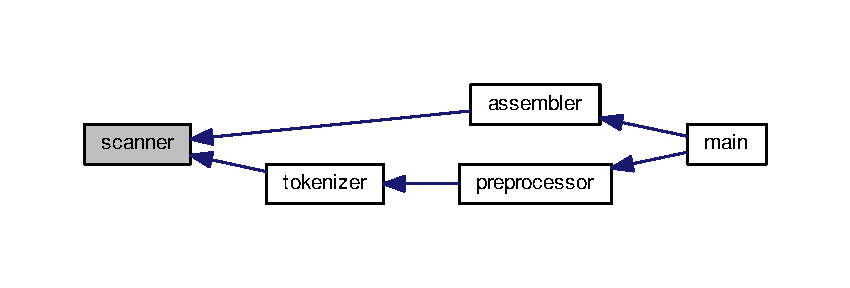
\includegraphics[width=304pt]{lexer_8cpp_a63ef6d488951c4541159fe0961565c4d_icgraph}
\end{center}
\end{figure}



\hypertarget{lexer_8h}{\section{Referência ao ficheiro lexer.\-h}
\label{lexer_8h}\index{lexer.\-h@{lexer.\-h}}
}
{\ttfamily \#include $<$string$>$}\\*
{\ttfamily \#include $<$vector$>$}\\*
{\ttfamily \#include \char`\"{}languagedefinition.\-h\char`\"{}}\\*
Diagrama de dependências de inclusão para lexer.\-h\-:\nopagebreak
\begin{figure}[H]
\begin{center}
\leavevmode
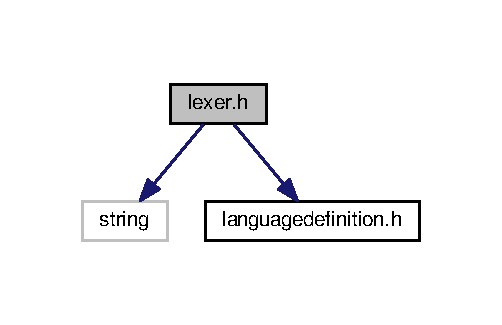
\includegraphics[width=304pt]{lexer_8h__incl}
\end{center}
\end{figure}
Este grafo mostra quais são os ficheiros que incluem directamente ou indirectamente este ficheiro\-:
\nopagebreak
\begin{figure}[H]
\begin{center}
\leavevmode
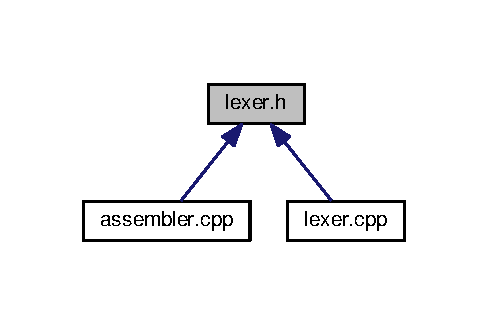
\includegraphics[width=350pt]{lexer_8h__dep__incl}
\end{center}
\end{figure}
\subsection*{Componentes}
\begin{DoxyCompactItemize}
\item 
struct \hyperlink{structtoken}{token}
\item 
struct \hyperlink{structinstruction_line}{instruction\-Line}
\end{DoxyCompactItemize}
\subsection*{Macros}
\begin{DoxyCompactItemize}
\item 
\#define \hyperlink{lexer_8h_a180873a64047585675744d9a3543109b}{D\-E\-B\-U\-G\-\_\-\-L\-E\-X\-E\-R}~0
\end{DoxyCompactItemize}
\subsection*{Enumerações}
\begin{DoxyCompactItemize}
\item 
enum \hyperlink{lexer_8h_aa520fbf142ba1e7e659590c07da31921}{Token\-Type} \{ \\*
\hyperlink{lexer_8h_aa520fbf142ba1e7e659590c07da31921a860a9a5cea93aed4f4a1ad272bd64694}{E\-R\-R\-C\-H\-A\-R} = -\/3, 
\hyperlink{lexer_8h_aa520fbf142ba1e7e659590c07da31921a1d52e71aa3a4ef78dca8e491eb29a073}{E\-R\-R\-N\-U\-M} = -\/2, 
\hyperlink{lexer_8h_aa520fbf142ba1e7e659590c07da31921aef2863a469df3ea6871d640e3669a2f2}{I\-N\-V\-A\-L\-I\-D} = -\/1, 
\hyperlink{lexer_8h_aa520fbf142ba1e7e659590c07da31921abc4f604c9e920142977c903ca8e10045}{S\-P\-C} = 0, 
\\*
\hyperlink{lexer_8h_aa520fbf142ba1e7e659590c07da31921af81277bcd86412fe04bb68718ea09392}{C\-O\-M\-M\-A} = 1, 
\hyperlink{lexer_8h_aa520fbf142ba1e7e659590c07da31921a29cf94637337909c3813bb50d6e9b3ee}{C\-O\-L\-O\-N} = 2, 
\hyperlink{lexer_8h_aa520fbf142ba1e7e659590c07da31921a55eebe3c7e08b49cd5969442f4f8c4ce}{S\-E\-M\-I\-C\-O\-L\-O\-N} = 3, 
\hyperlink{lexer_8h_aa520fbf142ba1e7e659590c07da31921a87fe59ef12c3d13dc2a4d14c9b16c1f9}{P\-L\-U\-S} = 4, 
\\*
\hyperlink{lexer_8h_aa520fbf142ba1e7e659590c07da31921af613d73b4e7b570ffd967df4a13c4225}{M\-I\-N\-U\-S} = 5, 
\hyperlink{lexer_8h_aa520fbf142ba1e7e659590c07da31921a959c8ebec5e5c8b2418482da8c0752ec}{L\-I\-N\-E\-\_\-\-E\-N\-D} = 6, 
\hyperlink{lexer_8h_aa520fbf142ba1e7e659590c07da31921a6efed498d807a51143031a4ac4427927}{S\-T\-R\-\_\-\-E\-N\-D} = 7, 
\hyperlink{lexer_8h_aa520fbf142ba1e7e659590c07da31921a9ed751de342a35124fd95551881b61f6}{N\-U\-M\-\_\-\-D\-E\-C} = 8, 
\\*
\hyperlink{lexer_8h_aa520fbf142ba1e7e659590c07da31921a95f9767a578c5cdafccdf25c9c35797c}{N\-U\-M\-\_\-\-H\-E\-X} = 9, 
\hyperlink{lexer_8h_aa520fbf142ba1e7e659590c07da31921a4ad40322037d6d371dca3e5cf993f5dc}{W\-O\-R\-D} = 10
 \}
\end{DoxyCompactItemize}
\subsection*{Funções}
\begin{DoxyCompactItemize}
\item 
\hyperlink{structtoken}{token} \hyperlink{lexer_8h_a63ef6d488951c4541159fe0961565c4d}{scanner} (std\-::string line, int $\ast$position)
\item 
vector$<$ \hyperlink{structtoken}{token} $>$ \hyperlink{lexer_8h_ab482a9701233ff4e5a0ffc1f75f9c41a}{tokenizer} (string line)
\end{DoxyCompactItemize}


\subsection{Documentação das macros}
\hypertarget{lexer_8h_a180873a64047585675744d9a3543109b}{\index{lexer.\-h@{lexer.\-h}!D\-E\-B\-U\-G\-\_\-\-L\-E\-X\-E\-R@{D\-E\-B\-U\-G\-\_\-\-L\-E\-X\-E\-R}}
\index{D\-E\-B\-U\-G\-\_\-\-L\-E\-X\-E\-R@{D\-E\-B\-U\-G\-\_\-\-L\-E\-X\-E\-R}!lexer.h@{lexer.\-h}}
\subsubsection[{D\-E\-B\-U\-G\-\_\-\-L\-E\-X\-E\-R}]{\setlength{\rightskip}{0pt plus 5cm}\#define D\-E\-B\-U\-G\-\_\-\-L\-E\-X\-E\-R~0}}\label{lexer_8h_a180873a64047585675744d9a3543109b}


Definido na linha 4 do ficheiro lexer.\-h.



\subsection{Documentação dos valores da enumeração}
\hypertarget{lexer_8h_aa520fbf142ba1e7e659590c07da31921}{\index{lexer.\-h@{lexer.\-h}!Token\-Type@{Token\-Type}}
\index{Token\-Type@{Token\-Type}!lexer.h@{lexer.\-h}}
\subsubsection[{Token\-Type}]{\setlength{\rightskip}{0pt plus 5cm}enum {\bf Token\-Type}}}\label{lexer_8h_aa520fbf142ba1e7e659590c07da31921}
Código para indentificar o tipo de token \begin{Desc}
\item[Valores da enumeração]\par
\begin{description}
\index{E\-R\-R\-C\-H\-A\-R@{E\-R\-R\-C\-H\-A\-R}!lexer.\-h@{lexer.\-h}}\index{lexer.\-h@{lexer.\-h}!E\-R\-R\-C\-H\-A\-R@{E\-R\-R\-C\-H\-A\-R}}\item[{\em 
\hypertarget{lexer_8h_aa520fbf142ba1e7e659590c07da31921a860a9a5cea93aed4f4a1ad272bd64694}{E\-R\-R\-C\-H\-A\-R}\label{lexer_8h_aa520fbf142ba1e7e659590c07da31921a860a9a5cea93aed4f4a1ad272bd64694}
}]Palavra mal formatada. \index{E\-R\-R\-N\-U\-M@{E\-R\-R\-N\-U\-M}!lexer.\-h@{lexer.\-h}}\index{lexer.\-h@{lexer.\-h}!E\-R\-R\-N\-U\-M@{E\-R\-R\-N\-U\-M}}\item[{\em 
\hypertarget{lexer_8h_aa520fbf142ba1e7e659590c07da31921a1d52e71aa3a4ef78dca8e491eb29a073}{E\-R\-R\-N\-U\-M}\label{lexer_8h_aa520fbf142ba1e7e659590c07da31921a1d52e71aa3a4ef78dca8e491eb29a073}
}]Número mal formatado. \index{I\-N\-V\-A\-L\-I\-D@{I\-N\-V\-A\-L\-I\-D}!lexer.\-h@{lexer.\-h}}\index{lexer.\-h@{lexer.\-h}!I\-N\-V\-A\-L\-I\-D@{I\-N\-V\-A\-L\-I\-D}}\item[{\em 
\hypertarget{lexer_8h_aa520fbf142ba1e7e659590c07da31921aef2863a469df3ea6871d640e3669a2f2}{I\-N\-V\-A\-L\-I\-D}\label{lexer_8h_aa520fbf142ba1e7e659590c07da31921aef2863a469df3ea6871d640e3669a2f2}
}]Token Inválido Genérico. \index{S\-P\-C@{S\-P\-C}!lexer.\-h@{lexer.\-h}}\index{lexer.\-h@{lexer.\-h}!S\-P\-C@{S\-P\-C}}\item[{\em 
\hypertarget{lexer_8h_aa520fbf142ba1e7e659590c07da31921abc4f604c9e920142977c903ca8e10045}{S\-P\-C}\label{lexer_8h_aa520fbf142ba1e7e659590c07da31921abc4f604c9e920142977c903ca8e10045}
}]Espaço em branco ' ' ou . \index{C\-O\-M\-M\-A@{C\-O\-M\-M\-A}!lexer.\-h@{lexer.\-h}}\index{lexer.\-h@{lexer.\-h}!C\-O\-M\-M\-A@{C\-O\-M\-M\-A}}\item[{\em 
\hypertarget{lexer_8h_aa520fbf142ba1e7e659590c07da31921af81277bcd86412fe04bb68718ea09392}{C\-O\-M\-M\-A}\label{lexer_8h_aa520fbf142ba1e7e659590c07da31921af81277bcd86412fe04bb68718ea09392}
}]\index{C\-O\-L\-O\-N@{C\-O\-L\-O\-N}!lexer.\-h@{lexer.\-h}}\index{lexer.\-h@{lexer.\-h}!C\-O\-L\-O\-N@{C\-O\-L\-O\-N}}\item[{\em 
\hypertarget{lexer_8h_aa520fbf142ba1e7e659590c07da31921a29cf94637337909c3813bb50d6e9b3ee}{C\-O\-L\-O\-N}\label{lexer_8h_aa520fbf142ba1e7e659590c07da31921a29cf94637337909c3813bb50d6e9b3ee}
}]\index{S\-E\-M\-I\-C\-O\-L\-O\-N@{S\-E\-M\-I\-C\-O\-L\-O\-N}!lexer.\-h@{lexer.\-h}}\index{lexer.\-h@{lexer.\-h}!S\-E\-M\-I\-C\-O\-L\-O\-N@{S\-E\-M\-I\-C\-O\-L\-O\-N}}\item[{\em 
\hypertarget{lexer_8h_aa520fbf142ba1e7e659590c07da31921a55eebe3c7e08b49cd5969442f4f8c4ce}{S\-E\-M\-I\-C\-O\-L\-O\-N}\label{lexer_8h_aa520fbf142ba1e7e659590c07da31921a55eebe3c7e08b49cd5969442f4f8c4ce}
}]\index{P\-L\-U\-S@{P\-L\-U\-S}!lexer.\-h@{lexer.\-h}}\index{lexer.\-h@{lexer.\-h}!P\-L\-U\-S@{P\-L\-U\-S}}\item[{\em 
\hypertarget{lexer_8h_aa520fbf142ba1e7e659590c07da31921a87fe59ef12c3d13dc2a4d14c9b16c1f9}{P\-L\-U\-S}\label{lexer_8h_aa520fbf142ba1e7e659590c07da31921a87fe59ef12c3d13dc2a4d14c9b16c1f9}
}]\index{M\-I\-N\-U\-S@{M\-I\-N\-U\-S}!lexer.\-h@{lexer.\-h}}\index{lexer.\-h@{lexer.\-h}!M\-I\-N\-U\-S@{M\-I\-N\-U\-S}}\item[{\em 
\hypertarget{lexer_8h_aa520fbf142ba1e7e659590c07da31921af613d73b4e7b570ffd967df4a13c4225}{M\-I\-N\-U\-S}\label{lexer_8h_aa520fbf142ba1e7e659590c07da31921af613d73b4e7b570ffd967df4a13c4225}
}]\index{L\-I\-N\-E\-\_\-\-E\-N\-D@{L\-I\-N\-E\-\_\-\-E\-N\-D}!lexer.\-h@{lexer.\-h}}\index{lexer.\-h@{lexer.\-h}!L\-I\-N\-E\-\_\-\-E\-N\-D@{L\-I\-N\-E\-\_\-\-E\-N\-D}}\item[{\em 
\hypertarget{lexer_8h_aa520fbf142ba1e7e659590c07da31921a959c8ebec5e5c8b2418482da8c0752ec}{L\-I\-N\-E\-\_\-\-E\-N\-D}\label{lexer_8h_aa520fbf142ba1e7e659590c07da31921a959c8ebec5e5c8b2418482da8c0752ec}
}]\index{S\-T\-R\-\_\-\-E\-N\-D@{S\-T\-R\-\_\-\-E\-N\-D}!lexer.\-h@{lexer.\-h}}\index{lexer.\-h@{lexer.\-h}!S\-T\-R\-\_\-\-E\-N\-D@{S\-T\-R\-\_\-\-E\-N\-D}}\item[{\em 
\hypertarget{lexer_8h_aa520fbf142ba1e7e659590c07da31921a6efed498d807a51143031a4ac4427927}{S\-T\-R\-\_\-\-E\-N\-D}\label{lexer_8h_aa520fbf142ba1e7e659590c07da31921a6efed498d807a51143031a4ac4427927}
}]\index{N\-U\-M\-\_\-\-D\-E\-C@{N\-U\-M\-\_\-\-D\-E\-C}!lexer.\-h@{lexer.\-h}}\index{lexer.\-h@{lexer.\-h}!N\-U\-M\-\_\-\-D\-E\-C@{N\-U\-M\-\_\-\-D\-E\-C}}\item[{\em 
\hypertarget{lexer_8h_aa520fbf142ba1e7e659590c07da31921a9ed751de342a35124fd95551881b61f6}{N\-U\-M\-\_\-\-D\-E\-C}\label{lexer_8h_aa520fbf142ba1e7e659590c07da31921a9ed751de342a35124fd95551881b61f6}
}]Número em decimal. \index{N\-U\-M\-\_\-\-H\-E\-X@{N\-U\-M\-\_\-\-H\-E\-X}!lexer.\-h@{lexer.\-h}}\index{lexer.\-h@{lexer.\-h}!N\-U\-M\-\_\-\-H\-E\-X@{N\-U\-M\-\_\-\-H\-E\-X}}\item[{\em 
\hypertarget{lexer_8h_aa520fbf142ba1e7e659590c07da31921a95f9767a578c5cdafccdf25c9c35797c}{N\-U\-M\-\_\-\-H\-E\-X}\label{lexer_8h_aa520fbf142ba1e7e659590c07da31921a95f9767a578c5cdafccdf25c9c35797c}
}]Número em hexadecimal. \index{W\-O\-R\-D@{W\-O\-R\-D}!lexer.\-h@{lexer.\-h}}\index{lexer.\-h@{lexer.\-h}!W\-O\-R\-D@{W\-O\-R\-D}}\item[{\em 
\hypertarget{lexer_8h_aa520fbf142ba1e7e659590c07da31921a4ad40322037d6d371dca3e5cf993f5dc}{W\-O\-R\-D}\label{lexer_8h_aa520fbf142ba1e7e659590c07da31921a4ad40322037d6d371dca3e5cf993f5dc}
}]\end{description}
\end{Desc}


Definido na linha 15 do ficheiro lexer.\-h.



\subsection{Documentação das funções}
\hypertarget{lexer_8h_a63ef6d488951c4541159fe0961565c4d}{\index{lexer.\-h@{lexer.\-h}!scanner@{scanner}}
\index{scanner@{scanner}!lexer.h@{lexer.\-h}}
\subsubsection[{scanner}]{\setlength{\rightskip}{0pt plus 5cm}{\bf token} scanner (
\begin{DoxyParamCaption}
\item[{std\-::string}]{line, }
\item[{int $\ast$}]{position}
\end{DoxyParamCaption}
)}}\label{lexer_8h_a63ef6d488951c4541159fe0961565c4d}
Verifica uma string em busca de tokens válidos 
\begin{DoxyParams}{Parâmetros}
{\em line} & String de Entrada \\
\hline
{\em position} & Posição \\
\hline
\end{DoxyParams}
\begin{DoxyReturn}{Retorna}
token 
\end{DoxyReturn}


Definido na linha 6 do ficheiro lexer.\-cpp.



Este é o diagrama das funções que utilizam esta função\-:
\nopagebreak
\begin{figure}[H]
\begin{center}
\leavevmode
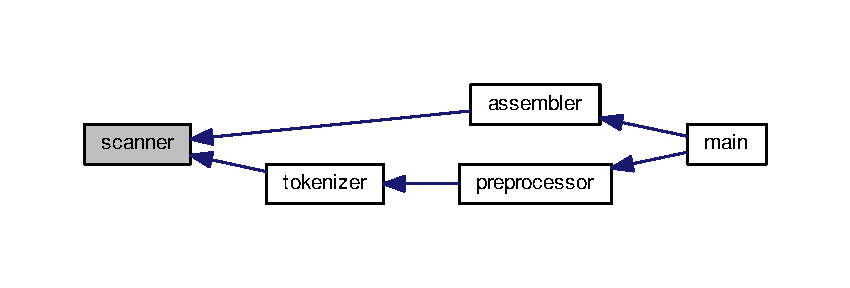
\includegraphics[width=350pt]{lexer_8h_a63ef6d488951c4541159fe0961565c4d_icgraph}
\end{center}
\end{figure}


\hypertarget{lexer_8h_ab482a9701233ff4e5a0ffc1f75f9c41a}{\index{lexer.\-h@{lexer.\-h}!tokenizer@{tokenizer}}
\index{tokenizer@{tokenizer}!lexer.h@{lexer.\-h}}
\subsubsection[{tokenizer}]{\setlength{\rightskip}{0pt plus 5cm}vector$<${\bf token}$>$ tokenizer (
\begin{DoxyParamCaption}
\item[{string}]{line}
\end{DoxyParamCaption}
)}}\label{lexer_8h_ab482a9701233ff4e5a0ffc1f75f9c41a}
Verifica uma string e retorna um vetor de tokens 
\begin{DoxyParams}{Parâmetros}
{\em line} & linha de entrada \\
\hline
\end{DoxyParams}
\begin{DoxyReturn}{Retorna}
tokens retornados 
\end{DoxyReturn}


Definido na linha 101 do ficheiro lexer.\-cpp.



Grafo de chamadas desta função\-:\nopagebreak
\begin{figure}[H]
\begin{center}
\leavevmode
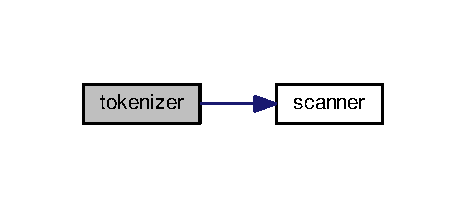
\includegraphics[width=224pt]{lexer_8h_ab482a9701233ff4e5a0ffc1f75f9c41a_cgraph}
\end{center}
\end{figure}




Este é o diagrama das funções que utilizam esta função\-:
\nopagebreak
\begin{figure}[H]
\begin{center}
\leavevmode
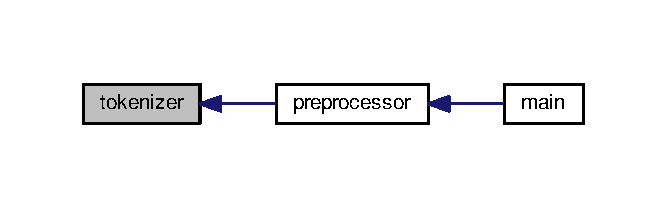
\includegraphics[width=320pt]{lexer_8h_ab482a9701233ff4e5a0ffc1f75f9c41a_icgraph}
\end{center}
\end{figure}



\hypertarget{main_8cpp}{\section{Referência ao ficheiro main.\-cpp}
\label{main_8cpp}\index{main.\-cpp@{main.\-cpp}}
}
{\ttfamily \#include $<$stdio.\-h$>$}\\*
{\ttfamily \#include $<$stdlib.\-h$>$}\\*
{\ttfamily \#include $<$ctype.\-h$>$}\\*
{\ttfamily \#include $<$string.\-h$>$}\\*
{\ttfamily \#include $<$unistd.\-h$>$}\\*
{\ttfamily \#include \char`\"{}mensagens.\-h\char`\"{}}\\*
{\ttfamily \#include \char`\"{}preprocessador.\-h\char`\"{}}\\*
{\ttfamily \#include \char`\"{}montador.\-h\char`\"{}}\\*
Diagrama de dependências de inclusão para main.\-cpp\-:
\nopagebreak
\begin{figure}[H]
\begin{center}
\leavevmode
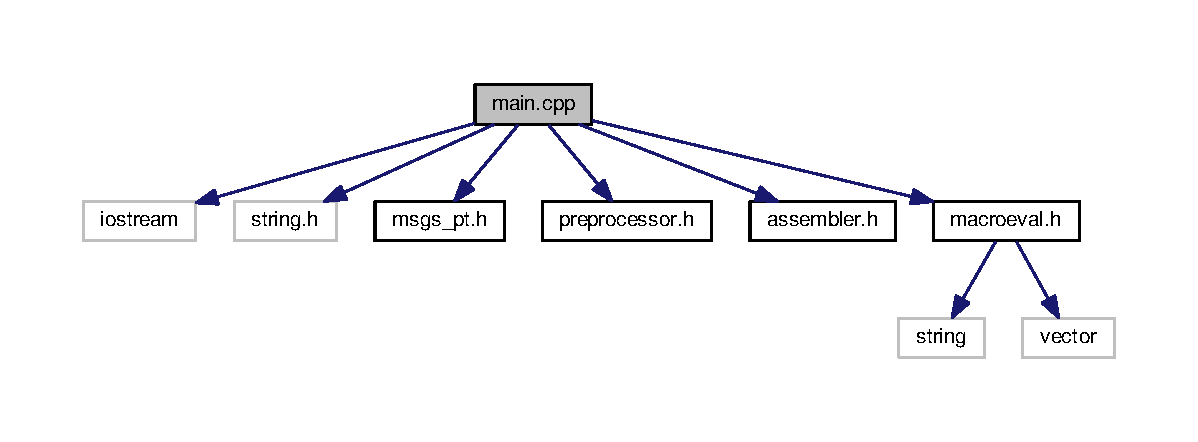
\includegraphics[width=350pt]{main_8cpp__incl}
\end{center}
\end{figure}
\subsection*{Funções}
\begin{DoxyCompactItemize}
\item 
int \hyperlink{main_8cpp_a3c04138a5bfe5d72780bb7e82a18e627}{main} (int argc, char $\ast$$\ast$argv)
\end{DoxyCompactItemize}


\subsection{Documentação das funções}
\hypertarget{main_8cpp_a3c04138a5bfe5d72780bb7e82a18e627}{\index{main.\-cpp@{main.\-cpp}!main@{main}}
\index{main@{main}!main.cpp@{main.\-cpp}}
\subsubsection[{main}]{\setlength{\rightskip}{0pt plus 5cm}int main (
\begin{DoxyParamCaption}
\item[{int}]{argc, }
\item[{char $\ast$$\ast$}]{argv}
\end{DoxyParamCaption}
)}}\label{main_8cpp_a3c04138a5bfe5d72780bb7e82a18e627}
Trabalho 1 -\/ Software Básico

\begin{DoxyAuthor}{Autores}
Rafael Lima e João Pedro Franch 
\end{DoxyAuthor}
\begin{DoxyVersion}{Versão}
0.\-2 
\end{DoxyVersion}
Pré Processamento (E\-Q\-U, I\-F) 

Definido na linha 18 do ficheiro main.\-cpp.



Grafo de chamadas desta função\-:
\nopagebreak
\begin{figure}[H]
\begin{center}
\leavevmode
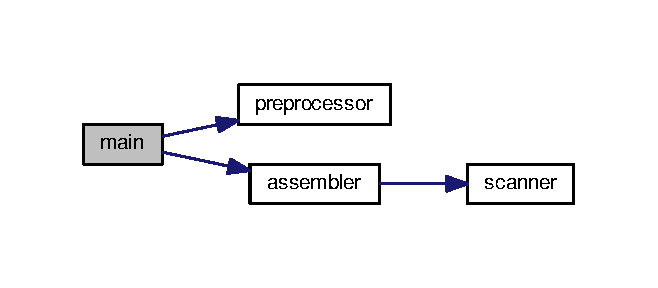
\includegraphics[width=240pt]{main_8cpp_a3c04138a5bfe5d72780bb7e82a18e627_cgraph}
\end{center}
\end{figure}



\hypertarget{msgs__pt_8h}{\section{Referência ao ficheiro msgs\-\_\-pt.\-h}
\label{msgs__pt_8h}\index{msgs\-\_\-pt.\-h@{msgs\-\_\-pt.\-h}}
}
Este grafo mostra quais são os ficheiros que incluem directamente ou indirectamente este ficheiro\-:\nopagebreak
\begin{figure}[H]
\begin{center}
\leavevmode
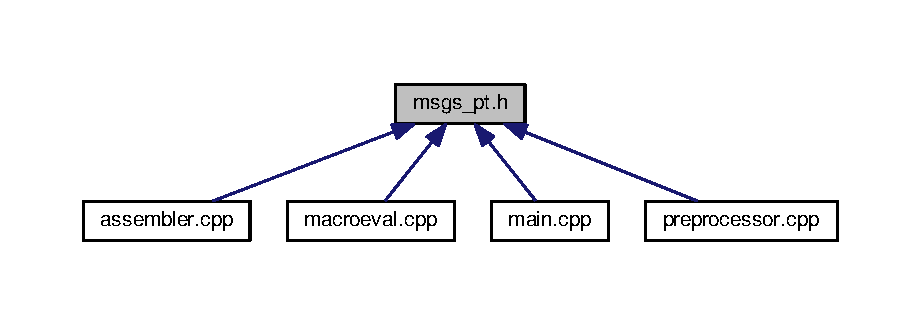
\includegraphics[width=350pt]{msgs__pt_8h__dep__incl}
\end{center}
\end{figure}
\subsection*{Macros}
\begin{DoxyCompactItemize}
\item 
\#define \hyperlink{msgs__pt_8h_a000d9d29df61eeb44781035464af5b3f}{M\-S\-G\-\_\-\-E\-R\-R}~\char`\"{}\textbackslash{}t\-E\-R\-R 9000\textbackslash{}n\char`\"{}
\item 
\#define \hyperlink{msgs__pt_8h_a2621adf4468e7cbf072ae921a989b5d0}{M\-S\-G\-\_\-\-E\-R\-R\-\_\-\-A\-R\-G\-U\-M\-E\-N\-T\-\_\-\-N\-U\-M\-B\-E\-R}~\char`\"{}\textbackslash{}t\-Número de argumentos invalido\textbackslash{}n\textbackslash{}t\-São necessarios 3 argumentos\-: o nome do file\-Name a ser compilado, a opcao e o nome do file\-Name objeto\textbackslash{}n\char`\"{}
\item 
\#define \hyperlink{msgs__pt_8h_a73e27a3d4632784bd871bdc3d4ffbe45}{M\-S\-G\-\_\-\-E\-R\-R\-\_\-\-I\-N\-V\-A\-L\-I\-D\-\_\-\-A\-R\-G\-U\-M\-E\-N\-T}~\char`\"{}\textbackslash{}t\-O segundo argumento esta mal formado\-:\textbackslash{}n\textbackslash{}t -\/p\-: pre-\/processado\textbackslash{}n\textbackslash{}t -\/m\-: file\-Name apos a resolucao das macros\textbackslash{}n\textbackslash{}t -\/o\-: para o file\-Name objeto final\textbackslash{}n\char`\"{}
\item 
\#define \hyperlink{msgs__pt_8h_a06a96287f556228b4efc43446ec84134}{M\-S\-G\-\_\-\-E\-R\-R\-\_\-\-F\-I\-L\-E}~\char`\"{}\textbackslash{}t\-Problemas ao abrir arquivo\textbackslash{}n\char`\"{}
\item 
\#define \hyperlink{msgs__pt_8h_aa9c72b3966543cca6087f95647022b8a}{M\-S\-G\-\_\-\-E\-R\-R\-\_\-\-I\-N\-V\-A\-L\-I\-D\-\_\-\-I\-N\-S\-T\-R\-U\-C\-T\-I\-O\-N}~\char`\"{}\textbackslash{}t\-Instrução Inválida\textbackslash{}n\textbackslash{}e\mbox{[}0\char`\"{}
\item 
\#define \hyperlink{msgs__pt_8h_a1f521fc4133c84430f6a83d481cc233f}{M\-S\-G\-\_\-\-E\-R\-R\-\_\-\-I\-N\-V\-A\-L\-I\-D\-\_\-\-T\-O\-K\-E\-N}~\char`\"{}\textbackslash{}t\-Token Inválido.\textbackslash{}n\char`\"{}
\item 
\#define \hyperlink{msgs__pt_8h_a25e6cdc1176e9281123cf738bac948ae}{M\-S\-G\-\_\-\-E\-R\-R\-\_\-\-L\-A\-B\-E\-L\-\_\-\-U\-N\-D\-E\-F\-I\-N\-E\-D}~\char`\"{}\textbackslash{}033\mbox{[}31m  -\/$>$ Rótulo Não definido\textbackslash{}033\mbox{[}0m\textbackslash{}n\char`\"{}
\item 
\#define \hyperlink{msgs__pt_8h_ab5d9ad3e68ee48b3a826ae801fe0c605}{M\-S\-G\-\_\-\-E\-R\-R\-\_\-\-M\-I\-S\-S\-I\-N\-G\-\_\-\-S\-E\-C\-T\-I\-O\-N\-\_\-\-T\-E\-X\-T}~\char`\"{}Linha 1\-: \textbackslash{}033\mbox{[}31m E\-R\-R\-O S\-I\-N\-TÁ\-T\-I\-C\-O\-: -\/$>$ Seção T\-E\-X\-T não declarada\textbackslash{}033\mbox{[}0m\textbackslash{}n\char`\"{}
\item 
\#define \hyperlink{msgs__pt_8h_a33fabfe7645f974b8beb74ca6fe409ec}{P\-R\-I\-N\-T\-\_\-\-E\-R\-R}(file\-Line, M\-S\-G)
\item 
\#define \hyperlink{msgs__pt_8h_ab660eca0513ca6bba1016b3aca4f2bf9}{P\-R\-I\-N\-T\-\_\-\-E\-R\-R\-\_\-\-T\-O\-K\-E\-N}(file\-Line, T\-O\-K)
\item 
\#define \hyperlink{msgs__pt_8h_acb4b755b37f4e2bec7953cb4bdab82d0}{P\-R\-I\-N\-T\-\_\-\-E\-R\-R\-\_\-\-I\-N\-S\-T\-R\-U\-C\-T\-I\-O\-N}(file\-Line, I\-N\-S\-T)
\item 
\#define \hyperlink{msgs__pt_8h_a81adad364cc31d62136f99d16be246d8}{P\-R\-I\-N\-T\-\_\-\-E\-R\-R\-\_\-\-L\-A\-B\-E\-L}(file\-Line, I\-N\-S\-T)
\item 
\#define \hyperlink{msgs__pt_8h_aa9e8177a6f52fdc518b4b001bf022a4a}{P\-R\-I\-N\-T\-\_\-\-E\-R\-R\-\_\-\-L\-A\-B\-E\-L\-\_\-\-U\-N\-D\-E\-F\-I\-N\-I\-E\-D}(file\-Line, I\-N\-S\-T)
\item 
\#define \hyperlink{msgs__pt_8h_a623c155fedd5a1c456f8c63b436c102f}{P\-R\-I\-N\-T\-\_\-\-E\-R\-R\-\_\-\-I\-F}(file\-Line, I\-N\-S\-T)
\item 
\#define \hyperlink{msgs__pt_8h_af6faed02032cd6305ee46046b040dba3}{P\-R\-I\-N\-T\-\_\-\-E\-R\-R\-\_\-\-L\-A\-B\-E\-L\-\_\-\-D\-U\-P\-L\-I\-C\-A\-T\-E\-D}(file\-Line, I\-N\-S\-T)
\item 
\#define \hyperlink{msgs__pt_8h_adac59590b65191e4efeb6b97c5e4b814}{P\-R\-I\-N\-T\-\_\-\-E\-R\-R\-\_\-\-I\-N\-V\-A\-L\-I\-D\-\_\-\-S\-E\-C\-T\-I\-O\-N}(file\-Line, I\-N\-S\-T)
\item 
\#define \hyperlink{msgs__pt_8h_a203775a37fc90d5aa4fde81cc63a6b7e}{P\-R\-I\-N\-T\-\_\-\-E\-R\-R\-\_\-\-W\-R\-O\-N\-G\-\_\-\-S\-E\-C\-T\-I\-O\-N\-\_\-\-D\-A\-T\-A\-\_\-\-I\-N\-S\-T\-R\-U\-C\-T\-I\-O\-N}(file\-Line, I\-N\-S\-T)
\item 
\#define \hyperlink{msgs__pt_8h_a8dee34733c6e908bded967f03121705f}{P\-R\-I\-N\-T\-\_\-\-E\-R\-R\-\_\-\-W\-R\-O\-N\-G\-\_\-\-S\-E\-C\-T\-I\-O\-N\-\_\-\-T\-E\-X\-T\-\_\-\-I\-N\-S\-T\-R\-U\-C\-T\-I\-O\-N}(file\-Line, I\-N\-S\-T)
\item 
\#define \hyperlink{msgs__pt_8h_a9f4e76369e81500b2abe3b783b9b0be3}{P\-R\-I\-N\-T\-\_\-\-E\-R\-R\-\_\-\-A\-R\-G\-\_\-\-N\-U\-M}(file\-Line, I\-N\-S\-T)
\item 
\#define \hyperlink{msgs__pt_8h_aef757d748dc80883f1145e6628c5348c}{P\-R\-I\-N\-T\-\_\-\-E\-R\-R\-\_\-\-A\-R\-G}(file\-Line, I\-N\-S\-T, A\-R\-G)
\item 
\#define \hyperlink{msgs__pt_8h_a82e7fabdec7483281a8c8641ac8b2646}{P\-R\-I\-N\-T\-\_\-\-E\-R\-R\-\_\-\-A\-R\-G\-\_\-\-T\-Y\-P\-E}(file\-Line, I\-N\-S\-T, A\-R\-G)
\item 
\#define \hyperlink{msgs__pt_8h_ae6c6a70c599abee737cbfec1285d88e3}{P\-R\-I\-N\-T\-\_\-\-E\-R\-R\-\_\-\-A\-R\-G\-\_\-\-T\-Y\-P\-E\-\_\-\-C\-O\-N\-S\-T}(file\-Line, I\-N\-S\-T, A\-R\-G)
\item 
\#define \hyperlink{msgs__pt_8h_a47671d7a51940c815dae870839ec5aae}{P\-R\-I\-N\-T\-\_\-\-E\-R\-R\-\_\-\-D\-I\-V0}(file\-Line, I\-N\-S\-T, A\-R\-G)
\end{DoxyCompactItemize}


\subsection{Documentação das macros}
\hypertarget{msgs__pt_8h_a000d9d29df61eeb44781035464af5b3f}{\index{msgs\-\_\-pt.\-h@{msgs\-\_\-pt.\-h}!M\-S\-G\-\_\-\-E\-R\-R@{M\-S\-G\-\_\-\-E\-R\-R}}
\index{M\-S\-G\-\_\-\-E\-R\-R@{M\-S\-G\-\_\-\-E\-R\-R}!msgs_pt.h@{msgs\-\_\-pt.\-h}}
\subsubsection[{M\-S\-G\-\_\-\-E\-R\-R}]{\setlength{\rightskip}{0pt plus 5cm}\#define M\-S\-G\-\_\-\-E\-R\-R~\char`\"{}\textbackslash{}t\-E\-R\-R 9000\textbackslash{}n\char`\"{}}}\label{msgs__pt_8h_a000d9d29df61eeb44781035464af5b3f}


Definido na linha 9 do ficheiro msgs\-\_\-pt.\-h.

\hypertarget{msgs__pt_8h_a2621adf4468e7cbf072ae921a989b5d0}{\index{msgs\-\_\-pt.\-h@{msgs\-\_\-pt.\-h}!M\-S\-G\-\_\-\-E\-R\-R\-\_\-\-A\-R\-G\-U\-M\-E\-N\-T\-\_\-\-N\-U\-M\-B\-E\-R@{M\-S\-G\-\_\-\-E\-R\-R\-\_\-\-A\-R\-G\-U\-M\-E\-N\-T\-\_\-\-N\-U\-M\-B\-E\-R}}
\index{M\-S\-G\-\_\-\-E\-R\-R\-\_\-\-A\-R\-G\-U\-M\-E\-N\-T\-\_\-\-N\-U\-M\-B\-E\-R@{M\-S\-G\-\_\-\-E\-R\-R\-\_\-\-A\-R\-G\-U\-M\-E\-N\-T\-\_\-\-N\-U\-M\-B\-E\-R}!msgs_pt.h@{msgs\-\_\-pt.\-h}}
\subsubsection[{M\-S\-G\-\_\-\-E\-R\-R\-\_\-\-A\-R\-G\-U\-M\-E\-N\-T\-\_\-\-N\-U\-M\-B\-E\-R}]{\setlength{\rightskip}{0pt plus 5cm}\#define M\-S\-G\-\_\-\-E\-R\-R\-\_\-\-A\-R\-G\-U\-M\-E\-N\-T\-\_\-\-N\-U\-M\-B\-E\-R~\char`\"{}\textbackslash{}t\-Número de argumentos invalido\textbackslash{}n\textbackslash{}t\-São necessarios 3 argumentos\-: o nome do file\-Name a ser compilado, a opcao e o nome do file\-Name objeto\textbackslash{}n\char`\"{}}}\label{msgs__pt_8h_a2621adf4468e7cbf072ae921a989b5d0}


Definido na linha 10 do ficheiro msgs\-\_\-pt.\-h.

\hypertarget{msgs__pt_8h_a06a96287f556228b4efc43446ec84134}{\index{msgs\-\_\-pt.\-h@{msgs\-\_\-pt.\-h}!M\-S\-G\-\_\-\-E\-R\-R\-\_\-\-F\-I\-L\-E@{M\-S\-G\-\_\-\-E\-R\-R\-\_\-\-F\-I\-L\-E}}
\index{M\-S\-G\-\_\-\-E\-R\-R\-\_\-\-F\-I\-L\-E@{M\-S\-G\-\_\-\-E\-R\-R\-\_\-\-F\-I\-L\-E}!msgs_pt.h@{msgs\-\_\-pt.\-h}}
\subsubsection[{M\-S\-G\-\_\-\-E\-R\-R\-\_\-\-F\-I\-L\-E}]{\setlength{\rightskip}{0pt plus 5cm}\#define M\-S\-G\-\_\-\-E\-R\-R\-\_\-\-F\-I\-L\-E~\char`\"{}\textbackslash{}t\-Problemas ao abrir arquivo\textbackslash{}n\char`\"{}}}\label{msgs__pt_8h_a06a96287f556228b4efc43446ec84134}


Definido na linha 12 do ficheiro msgs\-\_\-pt.\-h.

\hypertarget{msgs__pt_8h_a73e27a3d4632784bd871bdc3d4ffbe45}{\index{msgs\-\_\-pt.\-h@{msgs\-\_\-pt.\-h}!M\-S\-G\-\_\-\-E\-R\-R\-\_\-\-I\-N\-V\-A\-L\-I\-D\-\_\-\-A\-R\-G\-U\-M\-E\-N\-T@{M\-S\-G\-\_\-\-E\-R\-R\-\_\-\-I\-N\-V\-A\-L\-I\-D\-\_\-\-A\-R\-G\-U\-M\-E\-N\-T}}
\index{M\-S\-G\-\_\-\-E\-R\-R\-\_\-\-I\-N\-V\-A\-L\-I\-D\-\_\-\-A\-R\-G\-U\-M\-E\-N\-T@{M\-S\-G\-\_\-\-E\-R\-R\-\_\-\-I\-N\-V\-A\-L\-I\-D\-\_\-\-A\-R\-G\-U\-M\-E\-N\-T}!msgs_pt.h@{msgs\-\_\-pt.\-h}}
\subsubsection[{M\-S\-G\-\_\-\-E\-R\-R\-\_\-\-I\-N\-V\-A\-L\-I\-D\-\_\-\-A\-R\-G\-U\-M\-E\-N\-T}]{\setlength{\rightskip}{0pt plus 5cm}\#define M\-S\-G\-\_\-\-E\-R\-R\-\_\-\-I\-N\-V\-A\-L\-I\-D\-\_\-\-A\-R\-G\-U\-M\-E\-N\-T~\char`\"{}\textbackslash{}t\-O segundo argumento esta mal formado\-:\textbackslash{}n\textbackslash{}t -\/p\-: pre-\/processado\textbackslash{}n\textbackslash{}t -\/m\-: file\-Name apos a resolucao das macros\textbackslash{}n\textbackslash{}t -\/o\-: para o file\-Name objeto final\textbackslash{}n\char`\"{}}}\label{msgs__pt_8h_a73e27a3d4632784bd871bdc3d4ffbe45}


Definido na linha 11 do ficheiro msgs\-\_\-pt.\-h.

\hypertarget{msgs__pt_8h_aa9c72b3966543cca6087f95647022b8a}{\index{msgs\-\_\-pt.\-h@{msgs\-\_\-pt.\-h}!M\-S\-G\-\_\-\-E\-R\-R\-\_\-\-I\-N\-V\-A\-L\-I\-D\-\_\-\-I\-N\-S\-T\-R\-U\-C\-T\-I\-O\-N@{M\-S\-G\-\_\-\-E\-R\-R\-\_\-\-I\-N\-V\-A\-L\-I\-D\-\_\-\-I\-N\-S\-T\-R\-U\-C\-T\-I\-O\-N}}
\index{M\-S\-G\-\_\-\-E\-R\-R\-\_\-\-I\-N\-V\-A\-L\-I\-D\-\_\-\-I\-N\-S\-T\-R\-U\-C\-T\-I\-O\-N@{M\-S\-G\-\_\-\-E\-R\-R\-\_\-\-I\-N\-V\-A\-L\-I\-D\-\_\-\-I\-N\-S\-T\-R\-U\-C\-T\-I\-O\-N}!msgs_pt.h@{msgs\-\_\-pt.\-h}}
\subsubsection[{M\-S\-G\-\_\-\-E\-R\-R\-\_\-\-I\-N\-V\-A\-L\-I\-D\-\_\-\-I\-N\-S\-T\-R\-U\-C\-T\-I\-O\-N}]{\setlength{\rightskip}{0pt plus 5cm}\#define M\-S\-G\-\_\-\-E\-R\-R\-\_\-\-I\-N\-V\-A\-L\-I\-D\-\_\-\-I\-N\-S\-T\-R\-U\-C\-T\-I\-O\-N~\char`\"{}\textbackslash{}t\-Instrução Inválida\textbackslash{}n\textbackslash{}e\mbox{[}0\char`\"{}}}\label{msgs__pt_8h_aa9c72b3966543cca6087f95647022b8a}


Definido na linha 13 do ficheiro msgs\-\_\-pt.\-h.

\hypertarget{msgs__pt_8h_a1f521fc4133c84430f6a83d481cc233f}{\index{msgs\-\_\-pt.\-h@{msgs\-\_\-pt.\-h}!M\-S\-G\-\_\-\-E\-R\-R\-\_\-\-I\-N\-V\-A\-L\-I\-D\-\_\-\-T\-O\-K\-E\-N@{M\-S\-G\-\_\-\-E\-R\-R\-\_\-\-I\-N\-V\-A\-L\-I\-D\-\_\-\-T\-O\-K\-E\-N}}
\index{M\-S\-G\-\_\-\-E\-R\-R\-\_\-\-I\-N\-V\-A\-L\-I\-D\-\_\-\-T\-O\-K\-E\-N@{M\-S\-G\-\_\-\-E\-R\-R\-\_\-\-I\-N\-V\-A\-L\-I\-D\-\_\-\-T\-O\-K\-E\-N}!msgs_pt.h@{msgs\-\_\-pt.\-h}}
\subsubsection[{M\-S\-G\-\_\-\-E\-R\-R\-\_\-\-I\-N\-V\-A\-L\-I\-D\-\_\-\-T\-O\-K\-E\-N}]{\setlength{\rightskip}{0pt plus 5cm}\#define M\-S\-G\-\_\-\-E\-R\-R\-\_\-\-I\-N\-V\-A\-L\-I\-D\-\_\-\-T\-O\-K\-E\-N~\char`\"{}\textbackslash{}t\-Token Inválido.\textbackslash{}n\char`\"{}}}\label{msgs__pt_8h_a1f521fc4133c84430f6a83d481cc233f}


Definido na linha 14 do ficheiro msgs\-\_\-pt.\-h.

\hypertarget{msgs__pt_8h_a25e6cdc1176e9281123cf738bac948ae}{\index{msgs\-\_\-pt.\-h@{msgs\-\_\-pt.\-h}!M\-S\-G\-\_\-\-E\-R\-R\-\_\-\-L\-A\-B\-E\-L\-\_\-\-U\-N\-D\-E\-F\-I\-N\-E\-D@{M\-S\-G\-\_\-\-E\-R\-R\-\_\-\-L\-A\-B\-E\-L\-\_\-\-U\-N\-D\-E\-F\-I\-N\-E\-D}}
\index{M\-S\-G\-\_\-\-E\-R\-R\-\_\-\-L\-A\-B\-E\-L\-\_\-\-U\-N\-D\-E\-F\-I\-N\-E\-D@{M\-S\-G\-\_\-\-E\-R\-R\-\_\-\-L\-A\-B\-E\-L\-\_\-\-U\-N\-D\-E\-F\-I\-N\-E\-D}!msgs_pt.h@{msgs\-\_\-pt.\-h}}
\subsubsection[{M\-S\-G\-\_\-\-E\-R\-R\-\_\-\-L\-A\-B\-E\-L\-\_\-\-U\-N\-D\-E\-F\-I\-N\-E\-D}]{\setlength{\rightskip}{0pt plus 5cm}\#define M\-S\-G\-\_\-\-E\-R\-R\-\_\-\-L\-A\-B\-E\-L\-\_\-\-U\-N\-D\-E\-F\-I\-N\-E\-D~\char`\"{}\textbackslash{}033\mbox{[}31m  -\/$>$ Rótulo Não definido\textbackslash{}033\mbox{[}0m\textbackslash{}n\char`\"{}}}\label{msgs__pt_8h_a25e6cdc1176e9281123cf738bac948ae}


Definido na linha 15 do ficheiro msgs\-\_\-pt.\-h.

\hypertarget{msgs__pt_8h_ab5d9ad3e68ee48b3a826ae801fe0c605}{\index{msgs\-\_\-pt.\-h@{msgs\-\_\-pt.\-h}!M\-S\-G\-\_\-\-E\-R\-R\-\_\-\-M\-I\-S\-S\-I\-N\-G\-\_\-\-S\-E\-C\-T\-I\-O\-N\-\_\-\-T\-E\-X\-T@{M\-S\-G\-\_\-\-E\-R\-R\-\_\-\-M\-I\-S\-S\-I\-N\-G\-\_\-\-S\-E\-C\-T\-I\-O\-N\-\_\-\-T\-E\-X\-T}}
\index{M\-S\-G\-\_\-\-E\-R\-R\-\_\-\-M\-I\-S\-S\-I\-N\-G\-\_\-\-S\-E\-C\-T\-I\-O\-N\-\_\-\-T\-E\-X\-T@{M\-S\-G\-\_\-\-E\-R\-R\-\_\-\-M\-I\-S\-S\-I\-N\-G\-\_\-\-S\-E\-C\-T\-I\-O\-N\-\_\-\-T\-E\-X\-T}!msgs_pt.h@{msgs\-\_\-pt.\-h}}
\subsubsection[{M\-S\-G\-\_\-\-E\-R\-R\-\_\-\-M\-I\-S\-S\-I\-N\-G\-\_\-\-S\-E\-C\-T\-I\-O\-N\-\_\-\-T\-E\-X\-T}]{\setlength{\rightskip}{0pt plus 5cm}\#define M\-S\-G\-\_\-\-E\-R\-R\-\_\-\-M\-I\-S\-S\-I\-N\-G\-\_\-\-S\-E\-C\-T\-I\-O\-N\-\_\-\-T\-E\-X\-T~\char`\"{}Linha 1\-: \textbackslash{}033\mbox{[}31m E\-R\-R\-O S\-I\-N\-TÁ\-T\-I\-C\-O\-: -\/$>$ Seção T\-E\-X\-T não declarada\textbackslash{}033\mbox{[}0m\textbackslash{}n\char`\"{}}}\label{msgs__pt_8h_ab5d9ad3e68ee48b3a826ae801fe0c605}


Definido na linha 16 do ficheiro msgs\-\_\-pt.\-h.

\hypertarget{msgs__pt_8h_a33fabfe7645f974b8beb74ca6fe409ec}{\index{msgs\-\_\-pt.\-h@{msgs\-\_\-pt.\-h}!P\-R\-I\-N\-T\-\_\-\-E\-R\-R@{P\-R\-I\-N\-T\-\_\-\-E\-R\-R}}
\index{P\-R\-I\-N\-T\-\_\-\-E\-R\-R@{P\-R\-I\-N\-T\-\_\-\-E\-R\-R}!msgs_pt.h@{msgs\-\_\-pt.\-h}}
\subsubsection[{P\-R\-I\-N\-T\-\_\-\-E\-R\-R}]{\setlength{\rightskip}{0pt plus 5cm}\#define P\-R\-I\-N\-T\-\_\-\-E\-R\-R(
\begin{DoxyParamCaption}
\item[{}]{file\-Line, }
\item[{}]{M\-S\-G}
\end{DoxyParamCaption}
)}}\label{msgs__pt_8h_a33fabfe7645f974b8beb74ca6fe409ec}
{\bfseries Valor\-:}
\begin{DoxyCode}
cerr << \textcolor{stringliteral}{"\(\backslash\)n Linha "} << \(\backslash\)
                                          fileLine + 1 << \textcolor{stringliteral}{":\(\backslash\)033[31m ERRO:"} << \(\backslash\)
                                          MSG << \textcolor{stringliteral}{"\(\backslash\)033[0m\(\backslash\)n"}
\end{DoxyCode}


Definido na linha 19 do ficheiro msgs\-\_\-pt.\-h.

\hypertarget{msgs__pt_8h_aef757d748dc80883f1145e6628c5348c}{\index{msgs\-\_\-pt.\-h@{msgs\-\_\-pt.\-h}!P\-R\-I\-N\-T\-\_\-\-E\-R\-R\-\_\-\-A\-R\-G@{P\-R\-I\-N\-T\-\_\-\-E\-R\-R\-\_\-\-A\-R\-G}}
\index{P\-R\-I\-N\-T\-\_\-\-E\-R\-R\-\_\-\-A\-R\-G@{P\-R\-I\-N\-T\-\_\-\-E\-R\-R\-\_\-\-A\-R\-G}!msgs_pt.h@{msgs\-\_\-pt.\-h}}
\subsubsection[{P\-R\-I\-N\-T\-\_\-\-E\-R\-R\-\_\-\-A\-R\-G}]{\setlength{\rightskip}{0pt plus 5cm}\#define P\-R\-I\-N\-T\-\_\-\-E\-R\-R\-\_\-\-A\-R\-G(
\begin{DoxyParamCaption}
\item[{}]{file\-Line, }
\item[{}]{I\-N\-S\-T, }
\item[{}]{A\-R\-G}
\end{DoxyParamCaption}
)}}\label{msgs__pt_8h_aef757d748dc80883f1145e6628c5348c}
{\bfseries Valor\-:}
\begin{DoxyCode}
cerr << \textcolor{stringliteral}{"\(\backslash\)nLinha "} << \(\backslash\)
    fileLine +1 << \textcolor{stringliteral}{":\(\backslash\)033[31m ERRO ERRO SEMÂNTICO: \(\backslash\)033[0m\(\backslash\)""}<< string(INST) <<\(\backslash\)
    \textcolor{stringliteral}{"\(\backslash\)"\(\backslash\)033[31m  -> Argumento \(\backslash\)033[0m\(\backslash\)""}<< ARG <<\textcolor{stringliteral}{"\(\backslash\)"\(\backslash\)033[31m Inválido\(\backslash\)033[0m\(\backslash\)n"}
\end{DoxyCode}


Definido na linha 65 do ficheiro msgs\-\_\-pt.\-h.

\hypertarget{msgs__pt_8h_a9f4e76369e81500b2abe3b783b9b0be3}{\index{msgs\-\_\-pt.\-h@{msgs\-\_\-pt.\-h}!P\-R\-I\-N\-T\-\_\-\-E\-R\-R\-\_\-\-A\-R\-G\-\_\-\-N\-U\-M@{P\-R\-I\-N\-T\-\_\-\-E\-R\-R\-\_\-\-A\-R\-G\-\_\-\-N\-U\-M}}
\index{P\-R\-I\-N\-T\-\_\-\-E\-R\-R\-\_\-\-A\-R\-G\-\_\-\-N\-U\-M@{P\-R\-I\-N\-T\-\_\-\-E\-R\-R\-\_\-\-A\-R\-G\-\_\-\-N\-U\-M}!msgs_pt.h@{msgs\-\_\-pt.\-h}}
\subsubsection[{P\-R\-I\-N\-T\-\_\-\-E\-R\-R\-\_\-\-A\-R\-G\-\_\-\-N\-U\-M}]{\setlength{\rightskip}{0pt plus 5cm}\#define P\-R\-I\-N\-T\-\_\-\-E\-R\-R\-\_\-\-A\-R\-G\-\_\-\-N\-U\-M(
\begin{DoxyParamCaption}
\item[{}]{file\-Line, }
\item[{}]{I\-N\-S\-T}
\end{DoxyParamCaption}
)}}\label{msgs__pt_8h_a9f4e76369e81500b2abe3b783b9b0be3}
{\bfseries Valor\-:}
\begin{DoxyCode}
cerr << \textcolor{stringliteral}{"\(\backslash\)nLinha "} << \(\backslash\)
    fileLine +1 << \textcolor{stringliteral}{":\(\backslash\)033[31m ERRO SEMÂNTICO: \(\backslash\)033[0m\(\backslash\)""}<< string(INST) <<\(\backslash\)
    \textcolor{stringliteral}{"\(\backslash\)"\(\backslash\)033[31m  -> Número de argumentos Inválido.\(\backslash\)033[0m\(\backslash\)n"}
\end{DoxyCode}


Definido na linha 61 do ficheiro msgs\-\_\-pt.\-h.

\hypertarget{msgs__pt_8h_a82e7fabdec7483281a8c8641ac8b2646}{\index{msgs\-\_\-pt.\-h@{msgs\-\_\-pt.\-h}!P\-R\-I\-N\-T\-\_\-\-E\-R\-R\-\_\-\-A\-R\-G\-\_\-\-T\-Y\-P\-E@{P\-R\-I\-N\-T\-\_\-\-E\-R\-R\-\_\-\-A\-R\-G\-\_\-\-T\-Y\-P\-E}}
\index{P\-R\-I\-N\-T\-\_\-\-E\-R\-R\-\_\-\-A\-R\-G\-\_\-\-T\-Y\-P\-E@{P\-R\-I\-N\-T\-\_\-\-E\-R\-R\-\_\-\-A\-R\-G\-\_\-\-T\-Y\-P\-E}!msgs_pt.h@{msgs\-\_\-pt.\-h}}
\subsubsection[{P\-R\-I\-N\-T\-\_\-\-E\-R\-R\-\_\-\-A\-R\-G\-\_\-\-T\-Y\-P\-E}]{\setlength{\rightskip}{0pt plus 5cm}\#define P\-R\-I\-N\-T\-\_\-\-E\-R\-R\-\_\-\-A\-R\-G\-\_\-\-T\-Y\-P\-E(
\begin{DoxyParamCaption}
\item[{}]{file\-Line, }
\item[{}]{I\-N\-S\-T, }
\item[{}]{A\-R\-G}
\end{DoxyParamCaption}
)}}\label{msgs__pt_8h_a82e7fabdec7483281a8c8641ac8b2646}
{\bfseries Valor\-:}
\begin{DoxyCode}
cerr << \textcolor{stringliteral}{"\(\backslash\)nLinha "} << \(\backslash\)
    fileLine +1 << \textcolor{stringliteral}{":\(\backslash\)033[31m ERRO ERRO SEMÂNTICO: \(\backslash\)033[0m\(\backslash\)""}<< string(INST) <<\(\backslash\)
    \textcolor{stringliteral}{"\(\backslash\)"\(\backslash\)033[31m  -> Argumento \(\backslash\)033[0m\(\backslash\)""}<< ARG <<\textcolor{stringliteral}{"\(\backslash\)"\(\backslash\)033[31m com tipo inválido\(\backslash\)033[0m\(\backslash\)n"}
\end{DoxyCode}


Definido na linha 69 do ficheiro msgs\-\_\-pt.\-h.

\hypertarget{msgs__pt_8h_ae6c6a70c599abee737cbfec1285d88e3}{\index{msgs\-\_\-pt.\-h@{msgs\-\_\-pt.\-h}!P\-R\-I\-N\-T\-\_\-\-E\-R\-R\-\_\-\-A\-R\-G\-\_\-\-T\-Y\-P\-E\-\_\-\-C\-O\-N\-S\-T@{P\-R\-I\-N\-T\-\_\-\-E\-R\-R\-\_\-\-A\-R\-G\-\_\-\-T\-Y\-P\-E\-\_\-\-C\-O\-N\-S\-T}}
\index{P\-R\-I\-N\-T\-\_\-\-E\-R\-R\-\_\-\-A\-R\-G\-\_\-\-T\-Y\-P\-E\-\_\-\-C\-O\-N\-S\-T@{P\-R\-I\-N\-T\-\_\-\-E\-R\-R\-\_\-\-A\-R\-G\-\_\-\-T\-Y\-P\-E\-\_\-\-C\-O\-N\-S\-T}!msgs_pt.h@{msgs\-\_\-pt.\-h}}
\subsubsection[{P\-R\-I\-N\-T\-\_\-\-E\-R\-R\-\_\-\-A\-R\-G\-\_\-\-T\-Y\-P\-E\-\_\-\-C\-O\-N\-S\-T}]{\setlength{\rightskip}{0pt plus 5cm}\#define P\-R\-I\-N\-T\-\_\-\-E\-R\-R\-\_\-\-A\-R\-G\-\_\-\-T\-Y\-P\-E\-\_\-\-C\-O\-N\-S\-T(
\begin{DoxyParamCaption}
\item[{}]{file\-Line, }
\item[{}]{I\-N\-S\-T, }
\item[{}]{A\-R\-G}
\end{DoxyParamCaption}
)}}\label{msgs__pt_8h_ae6c6a70c599abee737cbfec1285d88e3}
{\bfseries Valor\-:}
\begin{DoxyCode}
cerr << \textcolor{stringliteral}{"\(\backslash\)nLinha "} << \(\backslash\)
    fileLine +1 << \textcolor{stringliteral}{":\(\backslash\)033[31m ERRO ERRO SEMÂNTICO: \(\backslash\)033[0m\(\backslash\)""}<< string(INST) <<\(\backslash\)
    \textcolor{stringliteral}{"\(\backslash\)"\(\backslash\)033[31m  -> Argumento \(\backslash\)033[0m\(\backslash\)""}<< ARG <<\textcolor{stringliteral}{"\(\backslash\)"\(\backslash\)033[31m com tipo inválido! Constante não é permitida
       como argumento de entrada.\(\backslash\)033[0m\(\backslash\)n"}
\end{DoxyCode}


Definido na linha 73 do ficheiro msgs\-\_\-pt.\-h.

\hypertarget{msgs__pt_8h_a47671d7a51940c815dae870839ec5aae}{\index{msgs\-\_\-pt.\-h@{msgs\-\_\-pt.\-h}!P\-R\-I\-N\-T\-\_\-\-E\-R\-R\-\_\-\-D\-I\-V0@{P\-R\-I\-N\-T\-\_\-\-E\-R\-R\-\_\-\-D\-I\-V0}}
\index{P\-R\-I\-N\-T\-\_\-\-E\-R\-R\-\_\-\-D\-I\-V0@{P\-R\-I\-N\-T\-\_\-\-E\-R\-R\-\_\-\-D\-I\-V0}!msgs_pt.h@{msgs\-\_\-pt.\-h}}
\subsubsection[{P\-R\-I\-N\-T\-\_\-\-E\-R\-R\-\_\-\-D\-I\-V0}]{\setlength{\rightskip}{0pt plus 5cm}\#define P\-R\-I\-N\-T\-\_\-\-E\-R\-R\-\_\-\-D\-I\-V0(
\begin{DoxyParamCaption}
\item[{}]{file\-Line, }
\item[{}]{I\-N\-S\-T, }
\item[{}]{A\-R\-G}
\end{DoxyParamCaption}
)}}\label{msgs__pt_8h_a47671d7a51940c815dae870839ec5aae}
{\bfseries Valor\-:}
\begin{DoxyCode}
cerr << \textcolor{stringliteral}{"\(\backslash\)nLinha "} << \(\backslash\)
    fileLine +1 << \textcolor{stringliteral}{":\(\backslash\)033[31m ERRO ERRO SEMÂNTICO: \(\backslash\)033[0m\(\backslash\)""}<< string(INST) <<\(\backslash\)
    \textcolor{stringliteral}{"\(\backslash\)"\(\backslash\)033[31m  -> Valor de \(\backslash\)033[0m\(\backslash\)""}<< ARG <<\textcolor{stringliteral}{"\(\backslash\)"\(\backslash\)033[31m Inválido. Dividindo Valor por zero!\(\backslash\)033[0m\(\backslash\)n"}
\end{DoxyCode}


Definido na linha 77 do ficheiro msgs\-\_\-pt.\-h.

\hypertarget{msgs__pt_8h_a623c155fedd5a1c456f8c63b436c102f}{\index{msgs\-\_\-pt.\-h@{msgs\-\_\-pt.\-h}!P\-R\-I\-N\-T\-\_\-\-E\-R\-R\-\_\-\-I\-F@{P\-R\-I\-N\-T\-\_\-\-E\-R\-R\-\_\-\-I\-F}}
\index{P\-R\-I\-N\-T\-\_\-\-E\-R\-R\-\_\-\-I\-F@{P\-R\-I\-N\-T\-\_\-\-E\-R\-R\-\_\-\-I\-F}!msgs_pt.h@{msgs\-\_\-pt.\-h}}
\subsubsection[{P\-R\-I\-N\-T\-\_\-\-E\-R\-R\-\_\-\-I\-F}]{\setlength{\rightskip}{0pt plus 5cm}\#define P\-R\-I\-N\-T\-\_\-\-E\-R\-R\-\_\-\-I\-F(
\begin{DoxyParamCaption}
\item[{}]{file\-Line, }
\item[{}]{I\-N\-S\-T}
\end{DoxyParamCaption}
)}}\label{msgs__pt_8h_a623c155fedd5a1c456f8c63b436c102f}
{\bfseries Valor\-:}
\begin{DoxyCode}
cerr << \textcolor{stringliteral}{"\(\backslash\)nLinha "} << \(\backslash\)
    fileLine +1 << \textcolor{stringliteral}{":\(\backslash\)033[31m ERRO SINTÁTICO: \(\backslash\)033[0m\(\backslash\)""}<< string(INST) <<\(\backslash\)
    \textcolor{stringliteral}{"\(\backslash\)"\(\backslash\)033[31m  -> Uso Incorreto da diretiva IF\(\backslash\)033[0m\(\backslash\)n"}
\end{DoxyCode}


Definido na linha 40 do ficheiro msgs\-\_\-pt.\-h.

\hypertarget{msgs__pt_8h_acb4b755b37f4e2bec7953cb4bdab82d0}{\index{msgs\-\_\-pt.\-h@{msgs\-\_\-pt.\-h}!P\-R\-I\-N\-T\-\_\-\-E\-R\-R\-\_\-\-I\-N\-S\-T\-R\-U\-C\-T\-I\-O\-N@{P\-R\-I\-N\-T\-\_\-\-E\-R\-R\-\_\-\-I\-N\-S\-T\-R\-U\-C\-T\-I\-O\-N}}
\index{P\-R\-I\-N\-T\-\_\-\-E\-R\-R\-\_\-\-I\-N\-S\-T\-R\-U\-C\-T\-I\-O\-N@{P\-R\-I\-N\-T\-\_\-\-E\-R\-R\-\_\-\-I\-N\-S\-T\-R\-U\-C\-T\-I\-O\-N}!msgs_pt.h@{msgs\-\_\-pt.\-h}}
\subsubsection[{P\-R\-I\-N\-T\-\_\-\-E\-R\-R\-\_\-\-I\-N\-S\-T\-R\-U\-C\-T\-I\-O\-N}]{\setlength{\rightskip}{0pt plus 5cm}\#define P\-R\-I\-N\-T\-\_\-\-E\-R\-R\-\_\-\-I\-N\-S\-T\-R\-U\-C\-T\-I\-O\-N(
\begin{DoxyParamCaption}
\item[{}]{file\-Line, }
\item[{}]{I\-N\-S\-T}
\end{DoxyParamCaption}
)}}\label{msgs__pt_8h_acb4b755b37f4e2bec7953cb4bdab82d0}
{\bfseries Valor\-:}
\begin{DoxyCode}
cerr << \textcolor{stringliteral}{"\(\backslash\)nLinha "} << \(\backslash\)
    fileLine +1 << \textcolor{stringliteral}{":\(\backslash\)033[31m ERRO SINTÁTICO: \(\backslash\)033[0m\(\backslash\)""}<< string(INST) <<\(\backslash\)
    \textcolor{stringliteral}{"\(\backslash\)"\(\backslash\)033[31m  -> Instrução Inválida\(\backslash\)033[0m\(\backslash\)n"}
\end{DoxyCode}


Definido na linha 27 do ficheiro msgs\-\_\-pt.\-h.

\hypertarget{msgs__pt_8h_adac59590b65191e4efeb6b97c5e4b814}{\index{msgs\-\_\-pt.\-h@{msgs\-\_\-pt.\-h}!P\-R\-I\-N\-T\-\_\-\-E\-R\-R\-\_\-\-I\-N\-V\-A\-L\-I\-D\-\_\-\-S\-E\-C\-T\-I\-O\-N@{P\-R\-I\-N\-T\-\_\-\-E\-R\-R\-\_\-\-I\-N\-V\-A\-L\-I\-D\-\_\-\-S\-E\-C\-T\-I\-O\-N}}
\index{P\-R\-I\-N\-T\-\_\-\-E\-R\-R\-\_\-\-I\-N\-V\-A\-L\-I\-D\-\_\-\-S\-E\-C\-T\-I\-O\-N@{P\-R\-I\-N\-T\-\_\-\-E\-R\-R\-\_\-\-I\-N\-V\-A\-L\-I\-D\-\_\-\-S\-E\-C\-T\-I\-O\-N}!msgs_pt.h@{msgs\-\_\-pt.\-h}}
\subsubsection[{P\-R\-I\-N\-T\-\_\-\-E\-R\-R\-\_\-\-I\-N\-V\-A\-L\-I\-D\-\_\-\-S\-E\-C\-T\-I\-O\-N}]{\setlength{\rightskip}{0pt plus 5cm}\#define P\-R\-I\-N\-T\-\_\-\-E\-R\-R\-\_\-\-I\-N\-V\-A\-L\-I\-D\-\_\-\-S\-E\-C\-T\-I\-O\-N(
\begin{DoxyParamCaption}
\item[{}]{file\-Line, }
\item[{}]{I\-N\-S\-T}
\end{DoxyParamCaption}
)}}\label{msgs__pt_8h_adac59590b65191e4efeb6b97c5e4b814}
{\bfseries Valor\-:}
\begin{DoxyCode}
cerr << \textcolor{stringliteral}{"\(\backslash\)nLinha "} << \(\backslash\)
    fileLine +1 << \textcolor{stringliteral}{":\(\backslash\)033[31m ERRO SINTÁTICO: \(\backslash\)033[0m\(\backslash\)""}<< string(INST) <<\(\backslash\)
    \textcolor{stringliteral}{"\(\backslash\)"\(\backslash\)033[31m  -> Definição de SECTION inválida, permitido somente TEXT ou DATA\(\backslash\)033[0m\(\backslash\)n"}
\end{DoxyCode}


Definido na linha 48 do ficheiro msgs\-\_\-pt.\-h.

\hypertarget{msgs__pt_8h_a81adad364cc31d62136f99d16be246d8}{\index{msgs\-\_\-pt.\-h@{msgs\-\_\-pt.\-h}!P\-R\-I\-N\-T\-\_\-\-E\-R\-R\-\_\-\-L\-A\-B\-E\-L@{P\-R\-I\-N\-T\-\_\-\-E\-R\-R\-\_\-\-L\-A\-B\-E\-L}}
\index{P\-R\-I\-N\-T\-\_\-\-E\-R\-R\-\_\-\-L\-A\-B\-E\-L@{P\-R\-I\-N\-T\-\_\-\-E\-R\-R\-\_\-\-L\-A\-B\-E\-L}!msgs_pt.h@{msgs\-\_\-pt.\-h}}
\subsubsection[{P\-R\-I\-N\-T\-\_\-\-E\-R\-R\-\_\-\-L\-A\-B\-E\-L}]{\setlength{\rightskip}{0pt plus 5cm}\#define P\-R\-I\-N\-T\-\_\-\-E\-R\-R\-\_\-\-L\-A\-B\-E\-L(
\begin{DoxyParamCaption}
\item[{}]{file\-Line, }
\item[{}]{I\-N\-S\-T}
\end{DoxyParamCaption}
)}}\label{msgs__pt_8h_a81adad364cc31d62136f99d16be246d8}
{\bfseries Valor\-:}
\begin{DoxyCode}
cerr << \textcolor{stringliteral}{"\(\backslash\)nLinha "} << \(\backslash\)
    fileLine +1 << \textcolor{stringliteral}{":\(\backslash\)033[31m ERRO SINTÁTICO: \(\backslash\)033[0m\(\backslash\)""}<< string(INST) <<\(\backslash\)
    \textcolor{stringliteral}{"\(\backslash\)"\(\backslash\)033[31m  -> Rótulo Inválido\(\backslash\)033[0m\(\backslash\)n"}
\end{DoxyCode}


Definido na linha 31 do ficheiro msgs\-\_\-pt.\-h.

\hypertarget{msgs__pt_8h_af6faed02032cd6305ee46046b040dba3}{\index{msgs\-\_\-pt.\-h@{msgs\-\_\-pt.\-h}!P\-R\-I\-N\-T\-\_\-\-E\-R\-R\-\_\-\-L\-A\-B\-E\-L\-\_\-\-D\-U\-P\-L\-I\-C\-A\-T\-E\-D@{P\-R\-I\-N\-T\-\_\-\-E\-R\-R\-\_\-\-L\-A\-B\-E\-L\-\_\-\-D\-U\-P\-L\-I\-C\-A\-T\-E\-D}}
\index{P\-R\-I\-N\-T\-\_\-\-E\-R\-R\-\_\-\-L\-A\-B\-E\-L\-\_\-\-D\-U\-P\-L\-I\-C\-A\-T\-E\-D@{P\-R\-I\-N\-T\-\_\-\-E\-R\-R\-\_\-\-L\-A\-B\-E\-L\-\_\-\-D\-U\-P\-L\-I\-C\-A\-T\-E\-D}!msgs_pt.h@{msgs\-\_\-pt.\-h}}
\subsubsection[{P\-R\-I\-N\-T\-\_\-\-E\-R\-R\-\_\-\-L\-A\-B\-E\-L\-\_\-\-D\-U\-P\-L\-I\-C\-A\-T\-E\-D}]{\setlength{\rightskip}{0pt plus 5cm}\#define P\-R\-I\-N\-T\-\_\-\-E\-R\-R\-\_\-\-L\-A\-B\-E\-L\-\_\-\-D\-U\-P\-L\-I\-C\-A\-T\-E\-D(
\begin{DoxyParamCaption}
\item[{}]{file\-Line, }
\item[{}]{I\-N\-S\-T}
\end{DoxyParamCaption}
)}}\label{msgs__pt_8h_af6faed02032cd6305ee46046b040dba3}
{\bfseries Valor\-:}
\begin{DoxyCode}
cerr << \textcolor{stringliteral}{"\(\backslash\)nLinha "} << \(\backslash\)
    fileLine +1 << \textcolor{stringliteral}{":\(\backslash\)033[31m ERRO SINTÁTICO: \(\backslash\)033[0m\(\backslash\)""}<< string(INST) <<\(\backslash\)
    \textcolor{stringliteral}{"\(\backslash\)"\(\backslash\)033[31m  -> Rótulo já definido\(\backslash\)033[0m\(\backslash\)n"}
\end{DoxyCode}


Definido na linha 44 do ficheiro msgs\-\_\-pt.\-h.

\hypertarget{msgs__pt_8h_aa9e8177a6f52fdc518b4b001bf022a4a}{\index{msgs\-\_\-pt.\-h@{msgs\-\_\-pt.\-h}!P\-R\-I\-N\-T\-\_\-\-E\-R\-R\-\_\-\-L\-A\-B\-E\-L\-\_\-\-U\-N\-D\-E\-F\-I\-N\-I\-E\-D@{P\-R\-I\-N\-T\-\_\-\-E\-R\-R\-\_\-\-L\-A\-B\-E\-L\-\_\-\-U\-N\-D\-E\-F\-I\-N\-I\-E\-D}}
\index{P\-R\-I\-N\-T\-\_\-\-E\-R\-R\-\_\-\-L\-A\-B\-E\-L\-\_\-\-U\-N\-D\-E\-F\-I\-N\-I\-E\-D@{P\-R\-I\-N\-T\-\_\-\-E\-R\-R\-\_\-\-L\-A\-B\-E\-L\-\_\-\-U\-N\-D\-E\-F\-I\-N\-I\-E\-D}!msgs_pt.h@{msgs\-\_\-pt.\-h}}
\subsubsection[{P\-R\-I\-N\-T\-\_\-\-E\-R\-R\-\_\-\-L\-A\-B\-E\-L\-\_\-\-U\-N\-D\-E\-F\-I\-N\-I\-E\-D}]{\setlength{\rightskip}{0pt plus 5cm}\#define P\-R\-I\-N\-T\-\_\-\-E\-R\-R\-\_\-\-L\-A\-B\-E\-L\-\_\-\-U\-N\-D\-E\-F\-I\-N\-I\-E\-D(
\begin{DoxyParamCaption}
\item[{}]{file\-Line, }
\item[{}]{I\-N\-S\-T}
\end{DoxyParamCaption}
)}}\label{msgs__pt_8h_aa9e8177a6f52fdc518b4b001bf022a4a}
{\bfseries Valor\-:}
\begin{DoxyCode}
cerr << \textcolor{stringliteral}{"\(\backslash\)nLinha "} << \(\backslash\)
    fileLine +1 << \textcolor{stringliteral}{":\(\backslash\)033[31m ERRO SINTÁTICO: \(\backslash\)033[0m\(\backslash\)""}<< string(INST) <<\(\backslash\)
    \textcolor{stringliteral}{"\(\backslash\)"\(\backslash\)033[31m  -> Rótulo Não Definido\(\backslash\)033[0m\(\backslash\)n"}
\end{DoxyCode}


Definido na linha 35 do ficheiro msgs\-\_\-pt.\-h.

\hypertarget{msgs__pt_8h_ab660eca0513ca6bba1016b3aca4f2bf9}{\index{msgs\-\_\-pt.\-h@{msgs\-\_\-pt.\-h}!P\-R\-I\-N\-T\-\_\-\-E\-R\-R\-\_\-\-T\-O\-K\-E\-N@{P\-R\-I\-N\-T\-\_\-\-E\-R\-R\-\_\-\-T\-O\-K\-E\-N}}
\index{P\-R\-I\-N\-T\-\_\-\-E\-R\-R\-\_\-\-T\-O\-K\-E\-N@{P\-R\-I\-N\-T\-\_\-\-E\-R\-R\-\_\-\-T\-O\-K\-E\-N}!msgs_pt.h@{msgs\-\_\-pt.\-h}}
\subsubsection[{P\-R\-I\-N\-T\-\_\-\-E\-R\-R\-\_\-\-T\-O\-K\-E\-N}]{\setlength{\rightskip}{0pt plus 5cm}\#define P\-R\-I\-N\-T\-\_\-\-E\-R\-R\-\_\-\-T\-O\-K\-E\-N(
\begin{DoxyParamCaption}
\item[{}]{file\-Line, }
\item[{}]{T\-O\-K}
\end{DoxyParamCaption}
)}}\label{msgs__pt_8h_ab660eca0513ca6bba1016b3aca4f2bf9}
{\bfseries Valor\-:}
\begin{DoxyCode}
cerr << \textcolor{stringliteral}{"\(\backslash\)nLinha "} << \(\backslash\)
                                          fileLine + 1 << \textcolor{stringliteral}{":\(\backslash\)033[31m ERRO LÉXICO: \(\backslash\)033[0m\(\backslash\)""} << \(\backslash\)
                                          TOK << \textcolor{stringliteral}{"\(\backslash\)"\(\backslash\)033[31m -> Token Inválido \(\backslash\)033[0m\(\backslash\)n"}
\end{DoxyCode}


Definido na linha 23 do ficheiro msgs\-\_\-pt.\-h.

\hypertarget{msgs__pt_8h_a203775a37fc90d5aa4fde81cc63a6b7e}{\index{msgs\-\_\-pt.\-h@{msgs\-\_\-pt.\-h}!P\-R\-I\-N\-T\-\_\-\-E\-R\-R\-\_\-\-W\-R\-O\-N\-G\-\_\-\-S\-E\-C\-T\-I\-O\-N\-\_\-\-D\-A\-T\-A\-\_\-\-I\-N\-S\-T\-R\-U\-C\-T\-I\-O\-N@{P\-R\-I\-N\-T\-\_\-\-E\-R\-R\-\_\-\-W\-R\-O\-N\-G\-\_\-\-S\-E\-C\-T\-I\-O\-N\-\_\-\-D\-A\-T\-A\-\_\-\-I\-N\-S\-T\-R\-U\-C\-T\-I\-O\-N}}
\index{P\-R\-I\-N\-T\-\_\-\-E\-R\-R\-\_\-\-W\-R\-O\-N\-G\-\_\-\-S\-E\-C\-T\-I\-O\-N\-\_\-\-D\-A\-T\-A\-\_\-\-I\-N\-S\-T\-R\-U\-C\-T\-I\-O\-N@{P\-R\-I\-N\-T\-\_\-\-E\-R\-R\-\_\-\-W\-R\-O\-N\-G\-\_\-\-S\-E\-C\-T\-I\-O\-N\-\_\-\-D\-A\-T\-A\-\_\-\-I\-N\-S\-T\-R\-U\-C\-T\-I\-O\-N}!msgs_pt.h@{msgs\-\_\-pt.\-h}}
\subsubsection[{P\-R\-I\-N\-T\-\_\-\-E\-R\-R\-\_\-\-W\-R\-O\-N\-G\-\_\-\-S\-E\-C\-T\-I\-O\-N\-\_\-\-D\-A\-T\-A\-\_\-\-I\-N\-S\-T\-R\-U\-C\-T\-I\-O\-N}]{\setlength{\rightskip}{0pt plus 5cm}\#define P\-R\-I\-N\-T\-\_\-\-E\-R\-R\-\_\-\-W\-R\-O\-N\-G\-\_\-\-S\-E\-C\-T\-I\-O\-N\-\_\-\-D\-A\-T\-A\-\_\-\-I\-N\-S\-T\-R\-U\-C\-T\-I\-O\-N(
\begin{DoxyParamCaption}
\item[{}]{file\-Line, }
\item[{}]{I\-N\-S\-T}
\end{DoxyParamCaption}
)}}\label{msgs__pt_8h_a203775a37fc90d5aa4fde81cc63a6b7e}
{\bfseries Valor\-:}
\begin{DoxyCode}
cerr << \textcolor{stringliteral}{"\(\backslash\)nLinha "} << \(\backslash\)
    fileLine +1 << \textcolor{stringliteral}{":\(\backslash\)033[31m ERRO SINTÁTICO: \(\backslash\)033[0m\(\backslash\)""}<< string(INST) <<\(\backslash\)
    \textcolor{stringliteral}{"\(\backslash\)"\(\backslash\)033[31m  -> Diretiva na Seção Errada! Deveria estar na seção DATA.\(\backslash\)033[0m\(\backslash\)n"}
\end{DoxyCode}


Definido na linha 52 do ficheiro msgs\-\_\-pt.\-h.

\hypertarget{msgs__pt_8h_a8dee34733c6e908bded967f03121705f}{\index{msgs\-\_\-pt.\-h@{msgs\-\_\-pt.\-h}!P\-R\-I\-N\-T\-\_\-\-E\-R\-R\-\_\-\-W\-R\-O\-N\-G\-\_\-\-S\-E\-C\-T\-I\-O\-N\-\_\-\-T\-E\-X\-T\-\_\-\-I\-N\-S\-T\-R\-U\-C\-T\-I\-O\-N@{P\-R\-I\-N\-T\-\_\-\-E\-R\-R\-\_\-\-W\-R\-O\-N\-G\-\_\-\-S\-E\-C\-T\-I\-O\-N\-\_\-\-T\-E\-X\-T\-\_\-\-I\-N\-S\-T\-R\-U\-C\-T\-I\-O\-N}}
\index{P\-R\-I\-N\-T\-\_\-\-E\-R\-R\-\_\-\-W\-R\-O\-N\-G\-\_\-\-S\-E\-C\-T\-I\-O\-N\-\_\-\-T\-E\-X\-T\-\_\-\-I\-N\-S\-T\-R\-U\-C\-T\-I\-O\-N@{P\-R\-I\-N\-T\-\_\-\-E\-R\-R\-\_\-\-W\-R\-O\-N\-G\-\_\-\-S\-E\-C\-T\-I\-O\-N\-\_\-\-T\-E\-X\-T\-\_\-\-I\-N\-S\-T\-R\-U\-C\-T\-I\-O\-N}!msgs_pt.h@{msgs\-\_\-pt.\-h}}
\subsubsection[{P\-R\-I\-N\-T\-\_\-\-E\-R\-R\-\_\-\-W\-R\-O\-N\-G\-\_\-\-S\-E\-C\-T\-I\-O\-N\-\_\-\-T\-E\-X\-T\-\_\-\-I\-N\-S\-T\-R\-U\-C\-T\-I\-O\-N}]{\setlength{\rightskip}{0pt plus 5cm}\#define P\-R\-I\-N\-T\-\_\-\-E\-R\-R\-\_\-\-W\-R\-O\-N\-G\-\_\-\-S\-E\-C\-T\-I\-O\-N\-\_\-\-T\-E\-X\-T\-\_\-\-I\-N\-S\-T\-R\-U\-C\-T\-I\-O\-N(
\begin{DoxyParamCaption}
\item[{}]{file\-Line, }
\item[{}]{I\-N\-S\-T}
\end{DoxyParamCaption}
)}}\label{msgs__pt_8h_a8dee34733c6e908bded967f03121705f}
{\bfseries Valor\-:}
\begin{DoxyCode}
cerr << \textcolor{stringliteral}{"\(\backslash\)nLinha "} << \(\backslash\)
    fileLine +1 << \textcolor{stringliteral}{":\(\backslash\)033[31m ERRO SINTÁTICO: \(\backslash\)033[0m\(\backslash\)""}<< string(INST) <<\(\backslash\)
    \textcolor{stringliteral}{"\(\backslash\)"\(\backslash\)033[31m  -> Instrução na Seção Errada! Deveria estar na seção TEXT.\(\backslash\)033[0m\(\backslash\)n"}
\end{DoxyCode}


Definido na linha 56 do ficheiro msgs\-\_\-pt.\-h.


\hypertarget{preprocessor_8cpp}{\section{Referência ao ficheiro preprocessor.\-cpp}
\label{preprocessor_8cpp}\index{preprocessor.\-cpp@{preprocessor.\-cpp}}
}
{\ttfamily \#include $<$sstream$>$}\\*
{\ttfamily \#include $<$iostream$>$}\\*
{\ttfamily \#include $<$fstream$>$}\\*
{\ttfamily \#include $<$string$>$}\\*
{\ttfamily \#include $<$algorithm$>$}\\*
{\ttfamily \#include $<$vector$>$}\\*
{\ttfamily \#include \char`\"{}msgs\-\_\-pt.\-h\char`\"{}}\\*
{\ttfamily \#include \char`\"{}preprocessor.\-h\char`\"{}}\\*
{\ttfamily \#include \char`\"{}lexer.\-h\char`\"{}}\\*
Diagrama de dependências de inclusão para preprocessor.\-cpp\-:
\nopagebreak
\begin{figure}[H]
\begin{center}
\leavevmode
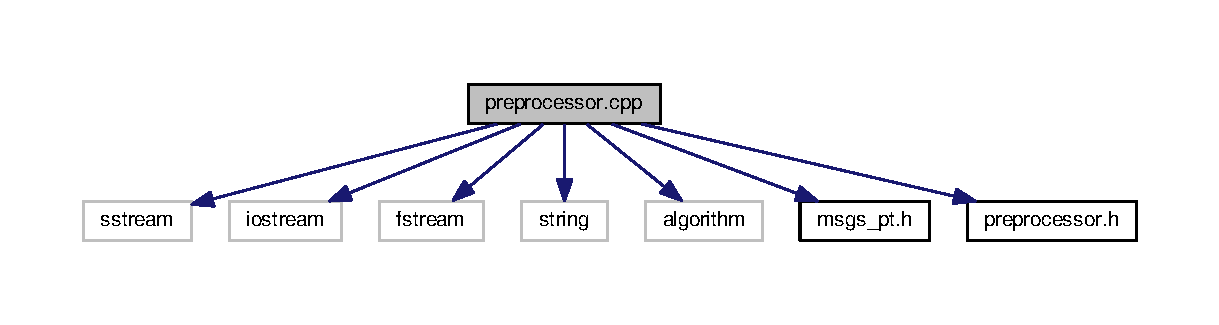
\includegraphics[width=350pt]{preprocessor_8cpp__incl}
\end{center}
\end{figure}
\subsection*{Funções}
\begin{DoxyCompactItemize}
\item 
int \hyperlink{preprocessor_8cpp_a64877d45066932f7594bb2ad347c1d26}{preprocessor} (int argc, char $\ast$$\ast$argv)
\end{DoxyCompactItemize}


\subsection{Documentação das funções}
\hypertarget{preprocessor_8cpp_a64877d45066932f7594bb2ad347c1d26}{\index{preprocessor.\-cpp@{preprocessor.\-cpp}!preprocessor@{preprocessor}}
\index{preprocessor@{preprocessor}!preprocessor.cpp@{preprocessor.\-cpp}}
\subsubsection[{preprocessor}]{\setlength{\rightskip}{0pt plus 5cm}int preprocessor (
\begin{DoxyParamCaption}
\item[{int}]{argc, }
\item[{char $\ast$$\ast$}]{argv}
\end{DoxyParamCaption}
)}}\label{preprocessor_8cpp_a64877d45066932f7594bb2ad347c1d26}


Definido na linha 18 do ficheiro preprocessor.\-cpp.



Grafo de chamadas desta função\-:
\nopagebreak
\begin{figure}[H]
\begin{center}
\leavevmode
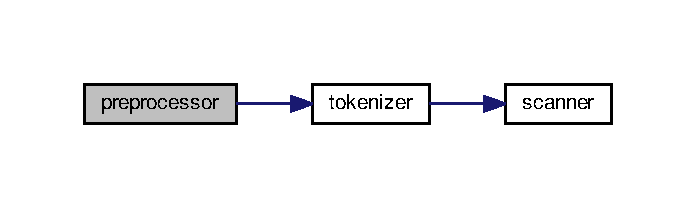
\includegraphics[width=334pt]{preprocessor_8cpp_a64877d45066932f7594bb2ad347c1d26_cgraph}
\end{center}
\end{figure}




Este é o diagrama das funções que utilizam esta função\-:\nopagebreak
\begin{figure}[H]
\begin{center}
\leavevmode
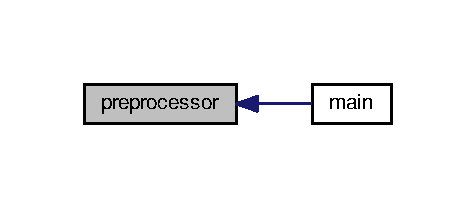
\includegraphics[width=228pt]{preprocessor_8cpp_a64877d45066932f7594bb2ad347c1d26_icgraph}
\end{center}
\end{figure}



\hypertarget{preprocessor_8h}{\section{Referência ao ficheiro preprocessor.\-h}
\label{preprocessor_8h}\index{preprocessor.\-h@{preprocessor.\-h}}
}
Este grafo mostra quais são os ficheiros que incluem directamente ou indirectamente este ficheiro\-:
\nopagebreak
\begin{figure}[H]
\begin{center}
\leavevmode
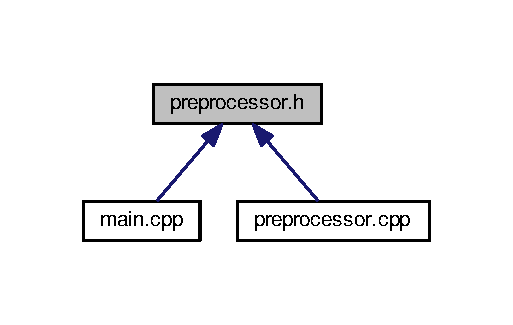
\includegraphics[width=246pt]{preprocessor_8h__dep__incl}
\end{center}
\end{figure}
\subsection*{Funções}
\begin{DoxyCompactItemize}
\item 
int \hyperlink{preprocessor_8h_a64877d45066932f7594bb2ad347c1d26}{preprocessor} (int argc, char $\ast$$\ast$argv)
\end{DoxyCompactItemize}


\subsection{Documentação das funções}
\hypertarget{preprocessor_8h_a64877d45066932f7594bb2ad347c1d26}{\index{preprocessor.\-h@{preprocessor.\-h}!preprocessor@{preprocessor}}
\index{preprocessor@{preprocessor}!preprocessor.h@{preprocessor.\-h}}
\subsubsection[{preprocessor}]{\setlength{\rightskip}{0pt plus 5cm}int preprocessor (
\begin{DoxyParamCaption}
\item[{int}]{argc, }
\item[{char $\ast$$\ast$}]{argv}
\end{DoxyParamCaption}
)}}\label{preprocessor_8h_a64877d45066932f7594bb2ad347c1d26}


Definido na linha 16 do ficheiro preprocessor.\-cpp.



Este é o diagrama das funções que utilizam esta função\-:\nopagebreak
\begin{figure}[H]
\begin{center}
\leavevmode
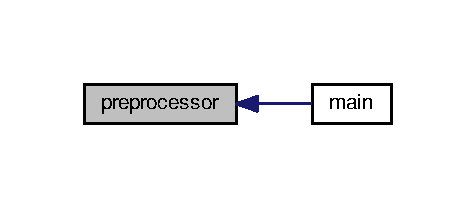
\includegraphics[width=228pt]{preprocessor_8h_a64877d45066932f7594bb2ad347c1d26_icgraph}
\end{center}
\end{figure}



%--- End generated contents ---

% Index
\newpage
\phantomsection
\addcontentsline{toc}{chapter}{Índice}
\printindex

\end{document}
